\chapter{Design}
\section{Struttura del Server}
Il server è strutturato principalmente in due macro-parti. Una parte del server si occupa di gestire tutte le richieste HTTP che provengono dal client, l'altra si occupa di gestire i messaggi relativi alle web-socket.

\subsection{Gestione delle Route}
Le route del server sono divise in delle categorie. La divisione è stata pensata solo per una separazione maggiore delle responsabilità, soprattutto per quanto riguarda la logica e il comportamento dei controller associati alle rotte.
Le rotte denotate con \textit{(auth middleware)} richiedono il token ottenuto durante la fase di login all'interno dell'header Authorization della richiesta.
\begin{itemize}
    \item Auth: Contiene tutte le rotte relative all'autenticazione.
    \begin{itemize}
        \item \textbf{POST - /auth/signup}: Crea un nuovo utente (se non già esistente) utilizzando username e password presenti nel body della richiesta.
        \item \textbf{POST - /auth/login} : Controlla se username e password coincidono con un qualche utente sul DB. In caso di esito positivo si ritorna un JWT.
        \item \textbf{GET - /profile \textit{(auth middleware)}}: Ritorna le informazioni dell'utente a partire dal token.
    \end{itemize}
    \item Notification:
    \begin{itemize}
        \item \textbf{GET - /notification \textit{(auth middleware)}}: Recupera le notifiche di un utente a partire dal suo token.
        \item \textbf{POST - /notification \textit{(auth middleware)}}: crea una nuova notifica per l'utente a cui appartiene il token presente nella richiesta.
        \item \textbf{DELETE - /notification:id \textit{(auth middleware)}}: cancella la notifica con l'id specificato nel parametro di query.
    \end{itemize}
            
    \item Resources: Contiene le rotte relative alle risorse che offre il sistema.
    \begin{itemize}
        \item \textbf{GET - /languages \textit{(auth middleware)}}: Recupera le lingue disponibili per il gioco.
        \item \textbf{GET - /dw/report:id \textit{(auth middleware)}}: scarica il report con l'id specificato nel parametro di query.
        \item \textbf{GET - /report \textit{(auth middleware)}}: recupera tutte le informazioni sui report di tutti i giocatori che hanno giocato nelle stesse partite in cui ha giocato l'utente che fa la richiesta,
    \end{itemize}
\end{itemize}


\subsection{Gestione delle Web Socket}
Quando il server riceve o invia un messaggio tramite websocket, esso è associato ad uno specifico canale.

\begin{itemize}
    \item \textbf{createLobby}: È il canale su cui vengono inviate le richieste da parte del client per creare nuove lobby. Il server risponde inviando il codice al client in caso di successo;
    \item \textbf{joinLobby}: È il canale su cui vengono inviate le richieste da parte del client per entare in una lobby. Il server aggiunge l'utente alla lobby ed invia come risposta tutte le informazioni relative alla lobby, come la lingua, il codice, la lista degli utenti etc;
    \item \textbf{startGame}: È il canale su cui vengono inviate le richieste da parte del client per iniziare una nuova partita. Solo l'admin della lobby può inviare un messaggio su questo canale. Il server si occupa di inviare un messaggio di broadcast a tutti gli utenti nella lobby, cambiando il loro stato interno e facendo iniziare la partita.
    \item \textbf{sentence}: È il canale su cui vengono inviate le frasi scritte dagli utenti durante una partita.
    \item \textbf{draw}: È il canale su cui vengono inviati i disegni fatti dagli utenti durante una partita.
    \item \textbf{forwardData}: È il canale utilizzato per gestire il sistema di ACK in modo da mantenere consistenza nello stato del sistema.
    \item \textbf{chat}: È il canale su cui vengono inviati i messaggi scritti fatti dagli utenti durante una partita.
    \item \textbf{endGame}: È il canale su cui vengono inviate le richieste da parte del client per iniziare terminare la partita ed uscire dalla fase di visualizzazione dei report. Solo un utente admin può inviare un messaggio su questo canale. Il server si occupa di inviare un messaggio di broadcast a tutti gli utenti nella lobby, cambiando il loro stato interno e spostandoli nella pagina di attesa della lobby.
    \item \textbf{disconnect}: È il canale su cui viene sempre inviato un messaggio se la socket viene chiusa (volontariamente o anche a causa di crash). Il canale è molto utile perché permette di mantenere consistenza in tutti i casi possibili, modificando lo stato e notificando in tempo reale la situazione anche ad eventuali altri utenti nella lobby.
\end{itemize}

\subsection{Stato del Server}
La gestione delle partite richiede l'utilizzo di alcune strutture dati che non hanno a che fare con i dati salvati all'interno del Database.
Nello specifico è molto importante modellare il sistema delle Lobby, i giocatori che ne fanno parte, ed i report dei giocatori che si arricchiscono mano a mano che la partita si avvicina alla sua fine. Inoltre si vorrebbero gestire i messaggi testuali che è possibile mandare mentre ci si trova all'interno di una lobby.\newline
Nello stato interno di Redux è presente solo una Mappa, le cui chiavi sono i codici univoci che identificano la lobby mentre i valori sono gli oggetti Lobby.\newline
Ad ogni giocatore viene anche collegata la relativa socket in modo da poter inviare messaggi al client dell'utente una volta recuperata.\newline
Lo stato delle lobby viene modificato solo attraverso gli handler delle socket, la gestione delle partite è infatti completamente gestita attraverso l'uso delle web-socket.\newline
Di seguito una breve descrizione delle classi del model:
\begin{itemize}
    \item \textbf{Lobby}: La classse principale del model che contiene tutte le altre. Contiene anche le informazioni generali della lobby come la lingua o se si tratta di una lobby pubblica o privata.
    \item \textbf{Player}: Rappresenta un giocatore all'interno della Lobby, il campo type denota se si tratta di un Admin, ovvero dell'utente che può far iniziare la partita.
    \item \textbf{ChatMessage}: Rappresenta un messaggio nella chat della Lobby.
    \item \textbf{Report}: Ad ogni utente è associato un Report, ovvero il foglio virtuale utilizzato nel gioco in cui vengono inserite le frasi e i disegni. Il report appartiene ad un determinato utente, ma viene anche passato ad altri utenti quando essi devono aggiungere contenuti.
    \item \textbf{Socket}: L'oggetto socket utilizzato dalla libreria socket.io associata all'utente.
    \item \textbf{Draw/Sentence}: Entrambe le classi sono in realtà stringhe. Draw è una stringa xml che rappresenta il disegno utilizzando lo standard SVG.
\end{itemize}

\begin{figure}[H]
    \caption{Diagramma delle classi del model del Server (in gioco)}
    \centering
    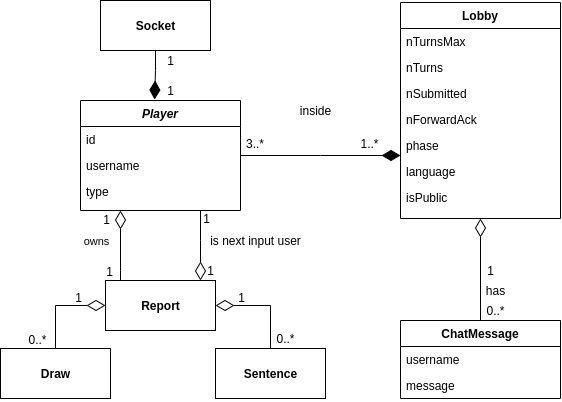
\includegraphics[width=400mm]{img/uml/guessr_server_model.png}
    \label{fig:guessr_server_model}
\end{figure}

\subsection{Gestione di una partita}
Per esplicare la gestione della comunicazione tra il server ed i vari client all'interno di una partita, verrà usato un diagramma di sequenza; in tale diagramma sono coinvolti il server, un client A che svolge il ruolo di Admin della lobby ed infine un secondo client B.\newline
Il gioco richiede in realtà un numero minimo di giocatori pari a 3, ma per semplificare la rappresentazione l'esempio coinvolge solo 2 giocatori.\newline

\noindent In rosso troviamo i messaggi inviati dall'Admin volti a modificare attivamente lo stato della lobby.\newline
In verde invece sono rappresentati i messaggi inviati dal server tramite i quali i vari client modificano le proprie UI, facendo progredire il gioco.\newline
In nero infine, sono presenti i messaggi dedicati allo scambio di frasi e disegni, input dei giocatori.

\begin{figure}[H]
    \caption{Diagramma di sequenza per lo svolgimento di una partita}
    \centering
    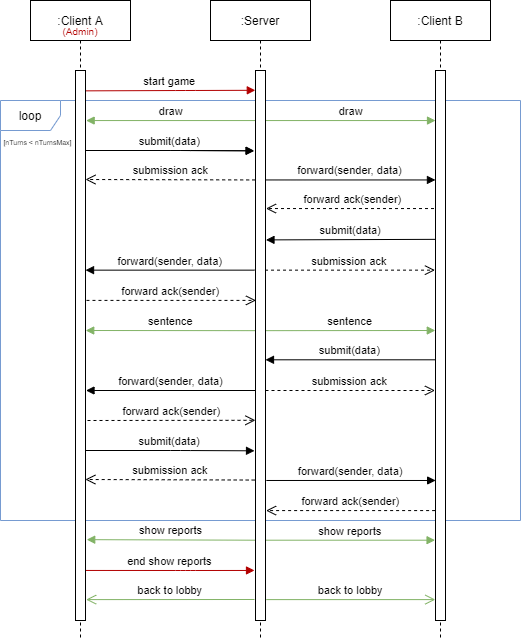
\includegraphics[width=400mm]{img/uml/guessr_game_sequence.png}
    \label{fig:guessr_game_sequence}
\end{figure}

\noindent Si presuppone che A e B si trovino all'interno di una lobby; durante la creazione di quest'ultima A ha impostato un numero di turni, ad esempio 3. Tale numero di turni verrà salvato nella variabile \textit{nTurnsMax}.\newline

\noindent A premerà  dunque il pulsante start game che scatenerà l'invio al server dell'omonimo messaggio; viene impostata a zero una variabile \textit{nTurns} la quale contiene il numero di turni trascorsi.\newline
Il server dunque esegue una broadcast inviando sul namespace \textit{draw} un messaggio. Alla ricezione del messaggio i client modificano la UI permettendo dunque ai giocatori di scrivere la loro prima frase.\newline

\noindent In questo esempio A scrive ed invia una frase prima di B; egli esegue dunque una submit inviando i suoi dati (la frase) al server che risponde gli con un \textit{submission ack}. Contemporaneamente il server invia inoltre, tramite \textit{forward}, i dati a tutti i membri della lobby TRANNE il mittente (A). Mentre B continua a scrivere la sua frase, il client in background salva i dati ricevuti ed invia un \textit{forward ack} al server.\newline

\noindent Ad un certo punto anche B invierà la sua frase, ripetendo messaggi analoghi a quelli sopra descritti.\newline

\noindent Dato N come il numero di giocatori, per verificare che tutti i giocatori abbiano inviato la loro frase e che ogni client disponga di una copia della frase di tutti gli altri giocatori, il server verifica di aver ricevuto un numero di forward ack pari ad N*(N-1).\newline
Il secondo termine nella moltiplicazione è minore di 1 rispetto al primo in quanto A salverà in locale la propria frase e dunque non riceverà un forward per la frase da lui inviata e, conseguentemente, non invierà un forward ack (in un esempio con 3 client A, B e C il server avrebbe ricevuto due ack per la frase di A, due per la frase di B ed altri 2 per la frase di C).\newline
Verificata tale condizione, il server invia in broadcast a tutti i giocatori un messaggio sul namespace \textit{sentence}, sentenziando la fine della fase dove i giocatori scrivono una frase.\newline

\noindent I client, ricevuto il messaggio, modificano nuovamente la loro UI per offrire la possibilità ad i giocatori di creare un disegno.\newline
Analogamente a prima, i giocatori inviano i loro dati (questa volta disegni) e, una volta ricevuto il giusto numero di forward ack, il server incrementa nTurns di 1; se nTurns < nTurnsMax, il server effettuerà una broadcast sul canale draw, sentenziando la fine della fase di disegno. I client modificheranno dunque nuovamente le loro UI per permettere l'input di una frase, ricominciando il ciclo.\newline

\noindent Nel caso invece in cui sia stato raggiunto il numero di turni impostati, il server eseguirà una broadcast sul namespace \textit{show reports}, segnalando ai client di mostrare a schermo i report di tutti gli utenti costruiti passo per passo tramite le precedenti forward.\newline

\noindent Quando l'Admin A lo riterrà più opportuno (solo egli avrà questa possibilità), segnalerà al server la sua volontà di terminare la visione dei report. Il server dunque eseguirà una broadcast sul namespace \textit{back to lobby}, riportando tutti i client alla lobby iniziale, dove l'Admin potrà nuovamente iniziare una nuova partita.\newline

\subsubsection{Possibile implementazione alternativa semplificata e vantaggi derivanti da quella adottata}
\noindent In un'implementazione alternativa, sarebbe stato possibile inviare ad ogni client solo il dato (frase o disegno) necessario per la prossima fase, inviando in broadcast solamente alla fine tutti i dati di tutti i report.\newline
Seppur tale implementazione sarebbe stata più semplice, ne avrebbe perso la qualità dell'esperienza utente, incrementando i tempi di attesa.\newline

\noindent Nella soluzione adottata, per ridurre i tempi derivanti dal download dei dati (specialmente dei disegni, che risultano molto più pesanti delle frasi), tale operazione viene effettuata in background sia mentre i giocatori più veloci nella creazione di frasi/disegni attendono quelli più lenti, sia mentre questi ultimi stanno per l'appunto completando il loro input.\newline

\noindent Nell'implementazione più semplice, invece, tutti i giocatori sarebbero stati costretti ad un'attesa più lunga dovuta ad una grande quantità di informazioni inviata ad ogni client. Per garantire la sincronia tra tutti i client, inoltre, anche i giocatori con una connessione veloce avrebbero dovuto attendere che quelli con una connessione lenta effettuassero il download di tutte le informazioni necessarie, vincolando l'attesa al client con la connessione più lenta.\newline

\noindent La soluzione adottata dunque elimina quasi totalmente il problema spalmando il download nel tempo e sfruttando i tempi morti che naturalmente si vengono a creare durante il gioco nell'attesa che tutti i giocatori abbiano terminato di creare il loro input.

\section{Struttura del Client}
Il client di GuessR è stato realizzato utilizzando il framework React.\newline

\noindent Il client è strutturato principalmente in tre macro-parti: Componenti, Stato ed Handler delle Socket.

\subsection{Componenti}
La struttura delle pagine dell'applicazione si trova dentro i componenti di React.
Per distinguere un componente da un normale file di Javascript basta guardare la lettera iniziale nel nome del file. Se è maiuscola si tratta di un componente React, altrimenti di un semplice modulo javascript.\newline
I componenti di React sono riutilizzabili a loro volta in altri componenti, permettendo di applicare il principio DRY anche in aspetti di strutturazione e non solo di logica.\newline
React nasce come framework per single page application. Per aggiungere altre route al sistema è necessaria la libreria \textit{React Router}, la quale mette a disposizione anche strumenti per effettuare il redirect utilizzando la logica base di React, andando a preservare lo stato interno del client.\newline
La suddivisione dei componenti è stata effettuata in base alla pagina in cui essi vengono utilizzati. I componenti comuni si trovano in una cartella denominata \textit{common}.
I componenti sono divisi per pagina.

\subsection{Stato del Client}
Lo stato dell'applicazione all'interno del client è stato incapsulato quasi completamente all'interno di Redux.\newline
Gli stati di React sono comunque stati utilizzati in maniera minore per gestire comportamenti della GUI o altri dettagli minori.\newline
All'interno dello stato di Redux del client sono incapsulati quattro oggetti:
\begin{itemize}
    \item \textbf{userInfo}: contiene tutte le informazioni dell'utente che ha effettuato l'accesso, in particolare:
    \begin{itemize}
        \item \textbf{id}: l'Id univoco dell'utente;
        \item \textbf{username}: il nome utente dell'utente;
        \item \textbf{token}: il web token dell'utente fornito dal server durante la fase di autenticazione;
        \item \textbf{notifications}: tutte le notifiche dell'utente;
    \end{itemize}
    \item \textbf{util}: contiene oggetti di utilità generale, in particolare:
    \begin{itemize}
        \item \textbf{languages}: l'elenco delle lingue disponibili per la creazione di una lobby;
        \item \textbf{socket}: la socket (oggetto della libreria socket.io) associata all'utente;
        \item \textbf{isLoading}: un campo booleano utile per far comparire una rotellina di caricamento a schermo in caso di attesa.
    \end{itemize}
    \item \textbf{lobby}:
    \begin{itemize}
        \item \textbf{settings}: contiene le impostazioni della lobby impostabili nel momento della creazione, in particolare:
            \begin{itemize}
                \item \textbf{isPublic}: true se la lobby è pubblica, false altrimenti;
                \item \textbf{nTurns}: il numero di turni che durerà la partita.
                \item \textbf{language}: la lingua che usata all'interno della lobbby;
            \end{itemize}
        \item \textbf{info}: contiene alcune informazioni della lobby, in particolare:
            \begin{itemize}
                \item \textbf{code}: il codice univoco della lobby;
                \item \textbf{users}: la lista degli utenti all'interno della lobby.
                \item \textbf{isMyRoleAdmin}: true se l'utente è admin della lobby, false altrimenti.
            \end{itemize}
        \item \textbf{status}: la fase in cui si trova la lobby.
        \item \textbf{waitingAllSubmit}: true se durante il gioco si sta ancora aspettando che almeno un utente invii la sua frase o il suo disegno.
        \item \textbf{messages}: l'elenco di messaggi presenti sulla chat.
        \item \textbf{receivedData}: la frase o il disegno ricevuto e su cui si baserà la risposta da inviare.
        \item \textbf{reports}: la lista di tutti i report che vengono popolati durante le fasi di gioco.
    \end{itemize}

    \item \textbf{previousReports}: contiene la lista dei report visionati nelle partite già giocate in precedenza.
\end{itemize}

\subsection{Gestione delle socket}
Quando il client riceve o invia un messaggio tramite websocket, esso è associato ad uno specifico canale.

\begin{itemize}
    \item \textbf{joined}: il canale su cui il server invia tutte le informazioni della lobby se l'utente è riuscito ad accedervi.
    \item \textbf{players}: il canale su cui il server invia tutte le informazioni riguardanti la connessione o la disconnesione da parte di altri giocatori all'interno della lobby.
    \item \textbf{chat}: il canale su cui il server invia tutte le informazioni riguardanti nuovi messaggi che vengono scritti all'interno della chat.
    \item \textbf{sentence}: il canale su cui il server invia la frase che l'utente ricevente dovrà disegnare.
    \item \textbf{draw}: il canale su cui il server invia il disegno che l'utente ricevente dovrà interpretare e descrivere con una frase.
    \item \textbf{forwardData}: il canale utilizzato per ricevere dati da parte del server riguardanti i report che vengono aggiornati.
    \item \textbf{showReport}: il canale su cui il server invia un messaggio quando la partita è finita e si possono visualizzare i risultati finali.
    \item \textbf{backToLobby}: il canale su cui il server invia la conferma per poter tornare nella fase di attesa all'interno della lobby una volta cambiato lo stato interno.
\end{itemize}

\section{Struttura del Database}
GuessR non richiede un Database particolarmente articolato.\newline
Una classe \textit{User} è necessaria per archiviare gli utenti e permettere la creazione di un sistema di autenticazione.
\begin{warn}[ATTENTZIONE:]
il campo password di User non contiene la password in chiaro, ma l'hash della password generata dal server.
\end{warn}
\begin{figure}[H]
    \caption{Diagramma delle classi della struttura del Database}
    \centering
    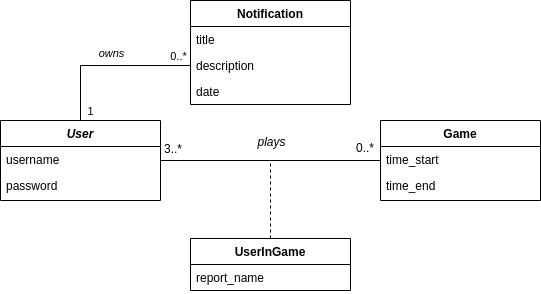
\includegraphics[width=400mm]{img/uml/guessr_db.png}
    \label{fig:wireframe_main_menu}
\end{figure}
Per aggiungere un sistema di notifiche all'applicazione è necessaria la creazione di una classe \textit{Notification}, legata a \textit{User} con cardinalità uno a molti, in quanto un utente può avere un numero qualsiasi di notifiche, ma la notifica è specifica per il singolo utente.\newline
La classe \textit{Game} rappresenta la partita a cui almeno tre utenti hanno preso parte. La cardinalità tra \textit{User} e \textit{Game} è molti a molti, in quanto ad una partita possono partecipare molti giocatori (almeno 3), mentre i giocatori possono aver giocato innumerevoli partite, o anche nessuna.\newline
La classe associativa \textit{UserInGame} rappresenta lo specifico utente che ha preso parte alla specifica partita. Il campo \textit{report\_name} è il nome del documento (situato nel server, è possibile scaricarlo attraverso il client) contenente il report finale.

\section{Interfaccia Utente}
\subsection{Wireframe}

\noindent In questa sezione verranno illustrati i Wireframe dell'applicazione, realizzati durante la fase di progettazione.
Tutte le schermate dell'applicazione sono state progettate con un'ottica mobile-first, ovvero puntando all'ottimizzazione del design su dispositivi mobili.\newline
In tutte le schermate compare una NavBar in cui compare il Logo dell'applicazione, una Label che indica il nome della pagina in cui ci si trova e un'icona rappresentante operazioni possibili per l'utente (per esempio il Logout).\newline
La prima pagina che compare quando si accde all'applicazione è la schermata di Autenticazione (Wireframe mancante). In questa schermata è possibile effettuare la registrazione di un nuovo account o il login. Qualora si effettuasse una registrazione verrà effettuato in automatico anche il Login. Inserendo le proprie credenziali in modo corretto e cliccando sul pulsante Login si potrà accedere al menù principale.\newline
In caso di credenziali sbagliate l'utente viene avvertito e viene invitato a provare di nuovo.

\noindent Nella schermata del menù Principale l'utente può cliccare su quattro pulsanti.
\begin{itemize}
    \item \textbf{Create Lobby}: Reindirizza l'utente alla pagina di creazione di una Lobby;
    \item \textbf{Join Random Lobby}: Fa comparire una schermata in cui l'utente deve inserire la propria lingua per poter entrare una Lobby casuale in cui gli utenti parleranno la sua stessa lingua;
    \item \textbf{Join Specific Game}: Fa comparire una schermata in cui l'utente deve inserire il codice identificativo di una lobby già creata;
    \item \textbf{Show previous Report}: Reindirizza l'utente alla pagina in cui può scaricare e consultare i report delle partite che ha giocato in passato.
\end{itemize}

\begin{figure}[H]
    \caption{Wireframe menu principale}
    \centering
    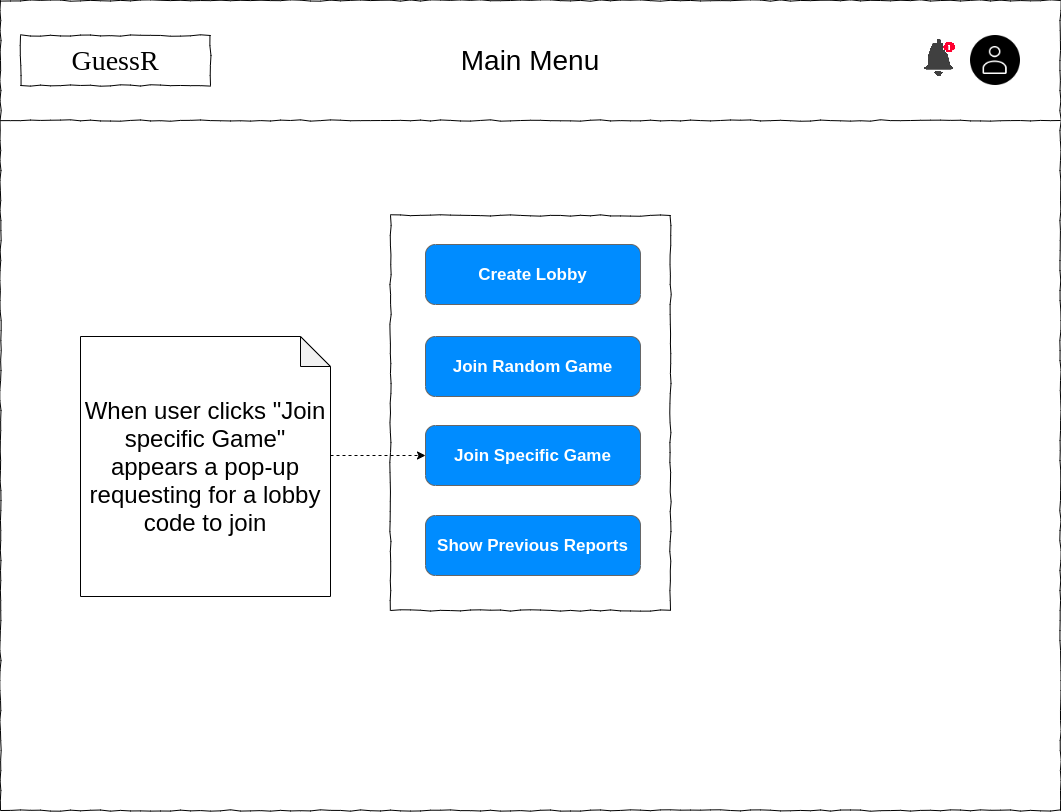
\includegraphics[width=400mm]{img/wireframes/main_menu.png}
    \label{fig:wireframe_main_menu}
\end{figure}

\noindent Premendo sul pulsante \textit{Create Lobby} compare la pagina di creazione di una Lobby. Questa pagina contiene un Form in cui è possibile impostare i parametri della Lobby. L'interruttore ``Set Visibilty" permette di impostare la visibilità della Lobby. Se si imposta la Lobby come privata solo gli utenti che posseggono il codice di accesso possono accedere. Se si imposta la lobby come pubblica qualsiasi utente potrà entrare nella Lobby.
È poi possibile inserire il numero di turni che si desidera giocare (un turno è definito come l'input sequenziale di una frase e un disegno da parte di tutti gli utenti). Infine è necessario selezionare la lingua in cui si vuole giocare tra le possibili offerte. Il pulsante \textit{"Create Lobby"} reindirizza l'utente alla pagina in cui attende che altri utenti accedano alla lobby per poter giocare.

\begin{figure}[H]
    \caption{Wireframe creazione lobby}
    \centering
    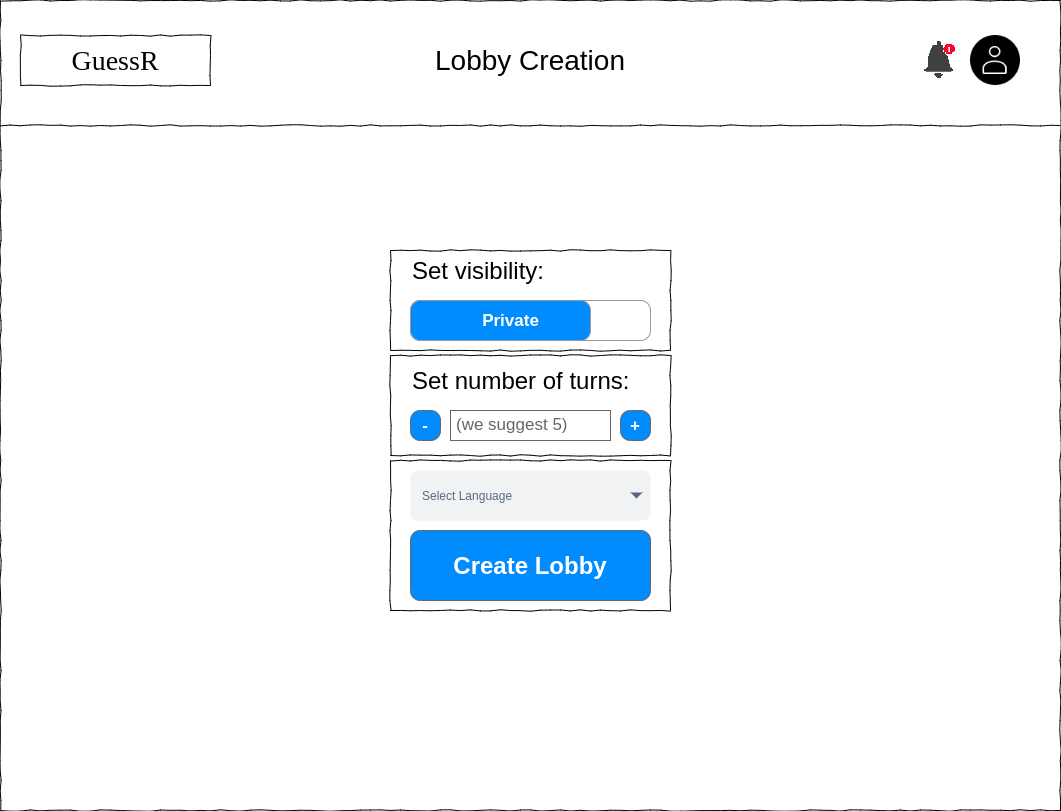
\includegraphics[width=400mm]{img/wireframes/lobby_creation.png}
    \label{fig:wireframe_lobby_creation}
\end{figure}

\noindent Nella schermata della Lobby creata compare il codice univoco assegnato alla Lobby sulla NavBar. Nella parte centrale dello schermo vengono illustrate le regole del gioco. Nella parte sinistra dello schermo compaiono i messaggi inviati dagli utenti ed il form utilizzato per mandarli. Nella parte destra dello schermo compare la lista dei giocatori all'interno della Lobby.
Infine, sotto le regole del gioco è presente un pulsante ``Exit Lobby" che se premuto fa uscire l'utente dalla Lobby. Un pulsante aggiuntivo ``Start Game" compare solo all'utente che ha creato la Lobby (l'utente di tipo Admin). Se premuto, questo pulsante reindirizza tutti gli utenti all'interno della Lobby alla schermata di Gioco.

\begin{figure}[H]
    \caption{Wireframe lobby}
    \centering
    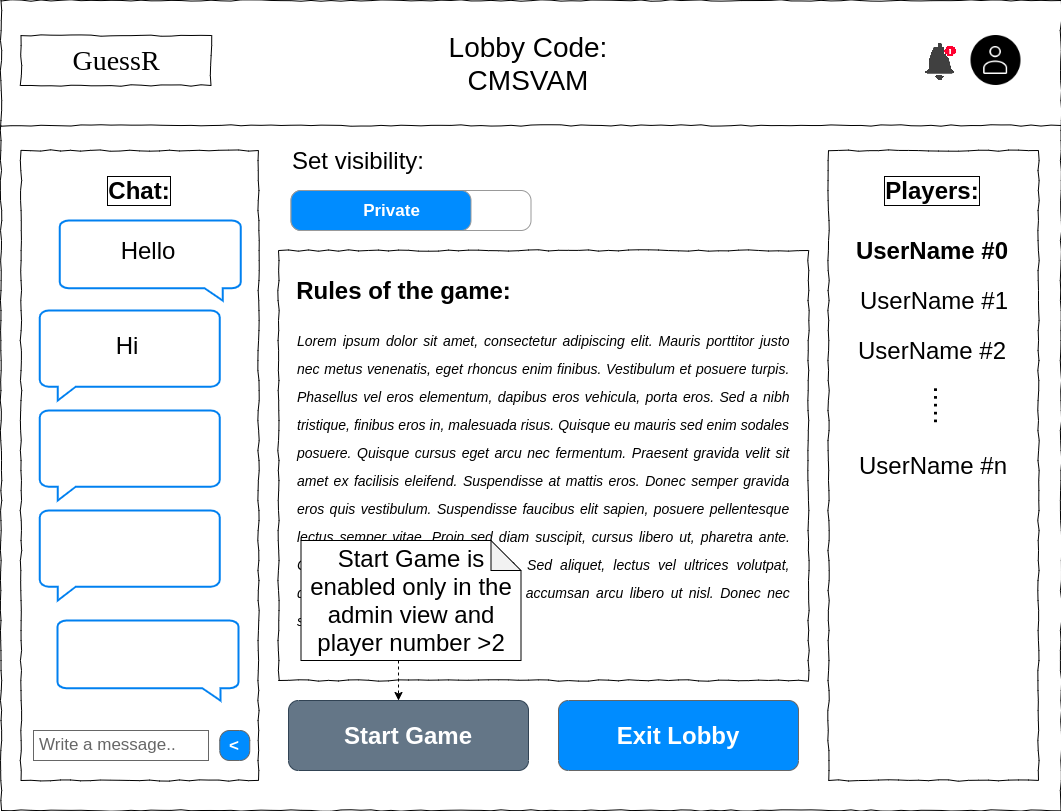
\includegraphics[width=400mm]{img/wireframes/in_lobby.png}
    \label{fig:wireframe_in_lobby}
\end{figure}

\noindent Nella schermata di gioco la parte destra e sinistra dello schermo rimane immutata rispetto alla pagine precedente. È quindi ancora possibile consultare ed inviare messaggi sulla chat e vedere i giocatori che stanno giocando.\newline
Sulla NavBar viene illustrata la fase di gioco.
\begin{itemize}
    \item Se la fase è \textit{``Sentence"} l'utente dovrà digitare una frase a suo piacimento (al primo turno o nel caso in cui non abbia ricevuto alcun disegno) o una frase che rappresenta in disegno che vede a schermo nel box di testo.
    \item Se la fase è \textit{``Draw"} l'utente dovrà disegnare come meglio possibile ciò che legge nella frase ricevuta.
    Il disegno va eseguito nell'apposito box bianco messo a disposizione.
\end{itemize}

\begin{figure}[H]
    \caption{Wireframe gioco}
    \centering
    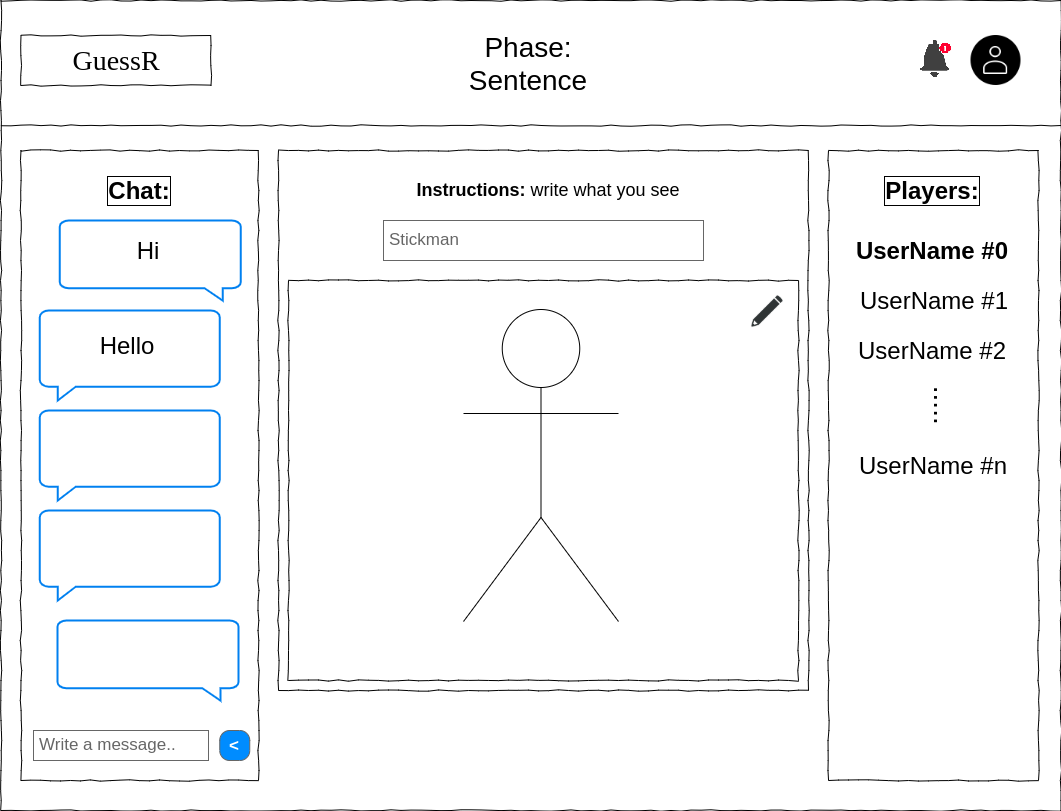
\includegraphics[width=400mm]{img/wireframes/in_game.png}
    \label{fig:wireframe_in_game_desktop}
\end{figure}

\noindent Quando il numero di turni finisce o un utente si disconnette tutti gli utenti vengono reindirizzati alla pagina in cui vengono visualizzati tutti i fogli (o report). Anche in questa pagina è presente un pulsante ``Exit Lobby" per uscire dalla Lobby. L'utente che ha creato la lobby ha a disposizione un ulteriore pulsante ``Back to Lobby" che reindirizza tutti gli utenti alla pagine in cui si attende che altri giocatori entrino nella Lobby. 

\begin{figure}[H]
    \caption{Wireframe gioco mobile}
    \centering
    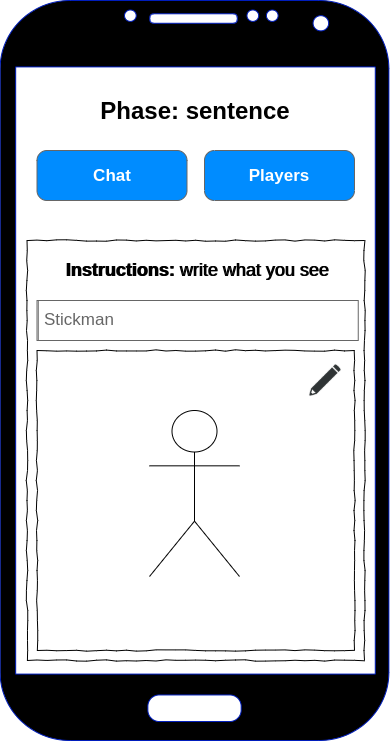
\includegraphics[width=175mm]{img/wireframes/mobile_in_game.png}
    \label{fig:wireframe_in_game_mobile}
\end{figure}

\noindent La maggior parte delle pagine contengono poco contenuto, fatta eccezione per le pagine in cui compaiono la chat e la lista degli utenti.\newline
Proprio questi due elementi, nella versione mobile dell'applicativo vengono condensati in due bottoni. Cliccando sui bottoni ``Chat" e ``Players" si apriranno dei pop-up che mostreranno le informazioni in un formato più consono alla dimensione dello schermo.

\subsection{Accessibilità}
Nello svolgimento del presente elaborato uno degli aspetti su cui ci siamo focalizzati maggiormente è quello dell'accessibilità, per poter permettere a più utenti possibile di interagire con l'applicativo giocando, e favorire l'inclusione anche di persone che fanno uso di screen reader. A tale scopo abbiamo cercato di uniformarci più possibile ai criteri di buona programmazione web e utilizzando delle best practices. \newline

\noindent Sia in fase di design dell'applicativo, design dell'interfaccia utente e della user experience, sia in fase di sviluppo abbiamo cercato di rendere l'applicativo quanto più accessibile, anche facendo ricorso a tool come axe devTools (set di tools leader nel settore, utilizzato anche da Microsoft e Google) che grazie alle sue linee guida ci ha permesso di focalizzare gli aspetti più importanti, come il giusto contrasto di colore, la zoomabilità delle pagine (soprattutto in caso di accesso da dispositivo mobile), le corrette proporzioni del testo e soprattutto una corretta integrazione di tag per agevolare l'utilizzo di screen readers o screen magnifiers.\newline

\noindent Guardando un risultato finale riteniamo di poter affermare dell'essere riusciti nell'intento di costruire un sito accessibile, in grado di includere persone ipovedenti o affette da daltonismo e adatto anche a chi ha necessità di ricorrere ad altri mezzi per la navigazione.

\subsection{Schermate finali}
Seguono gli screen relativi alle schermate di gioco definitive, effettuati durante una effettiva partita tra le personas descritte precedentemente.

\begin{figure}[H]
  \centering
  \begin{minipage}[b]{0.75\textwidth}
    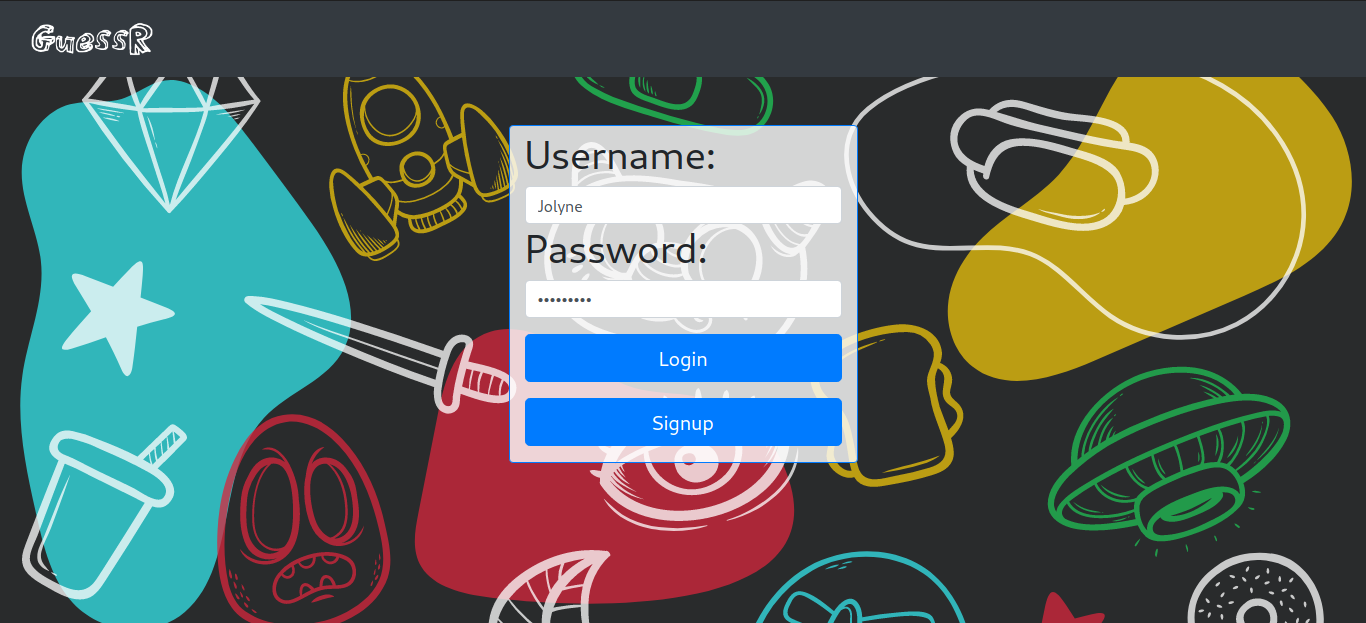
\includegraphics[width=\textwidth]{img/screen/Login.png}
  \end{minipage}
  \hfill
  \begin{minipage}[b]{0.2\textwidth}
    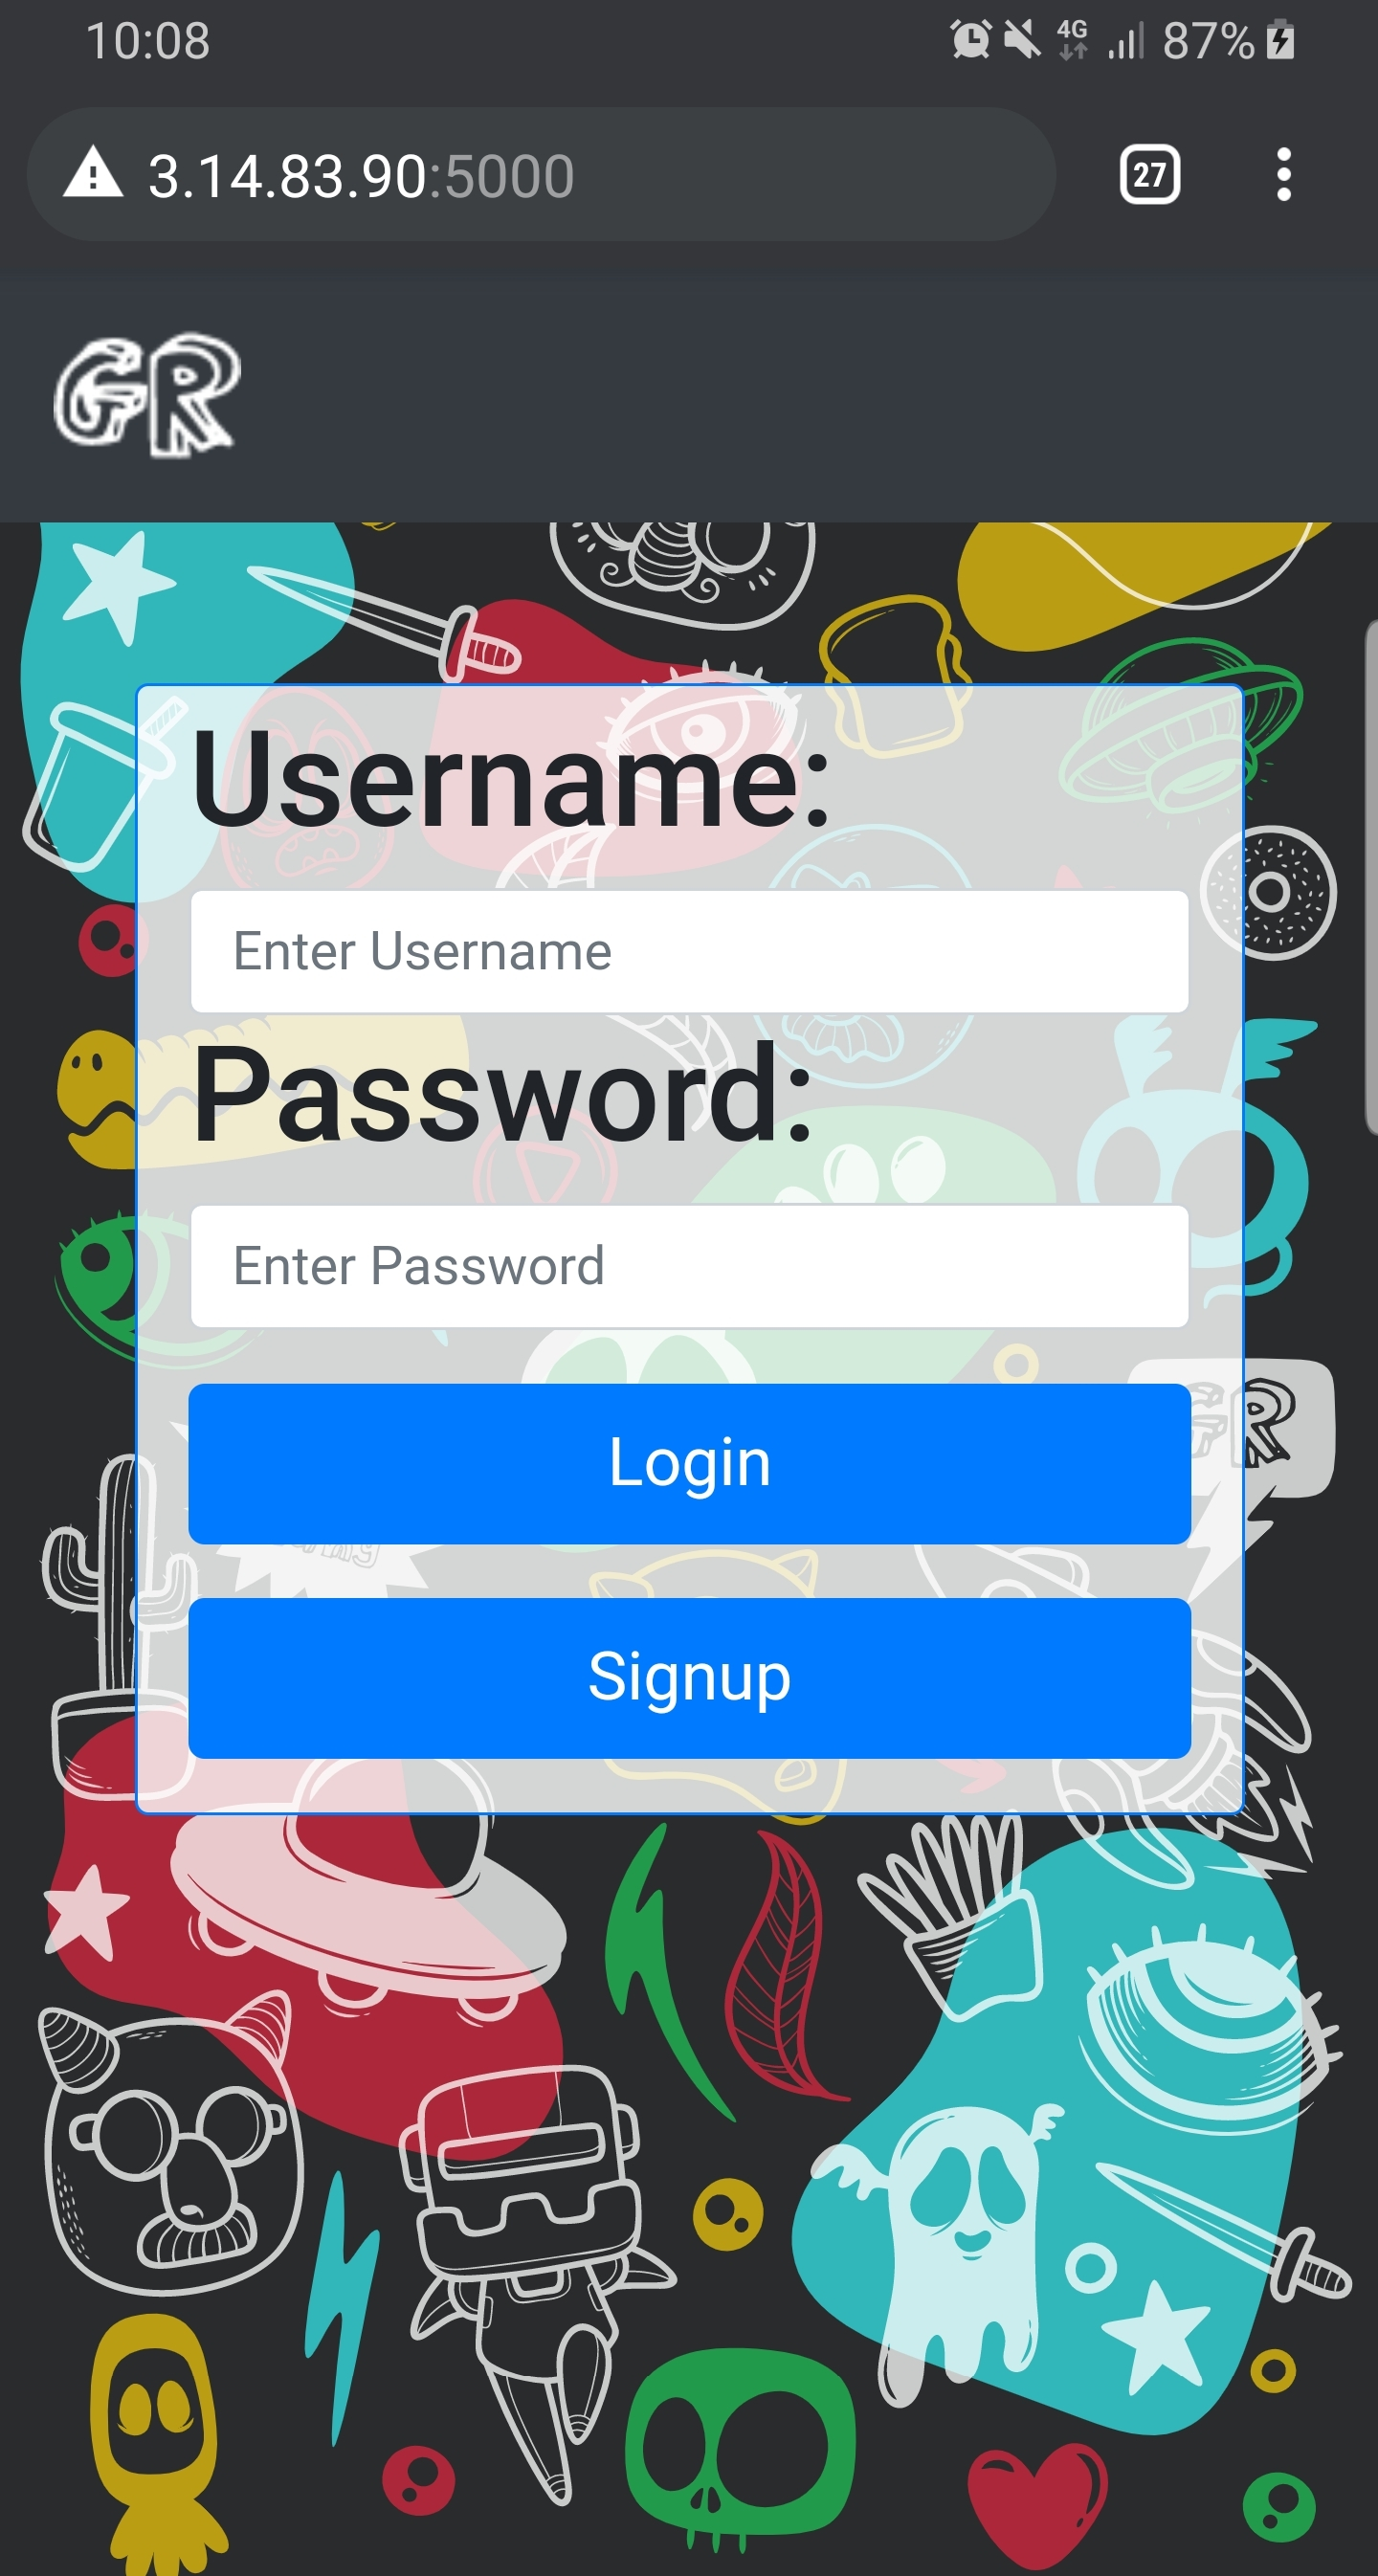
\includegraphics[width=\textwidth]{img/screen/M login.jpg}
  \end{minipage}
  \caption{Schermate di Login (Desktop e Mobile)}
\end{figure}

\noindent La schermata di login presenta una form per l'autenticazione dell'utente, in cui dovrà essere inserita uno username univoco ed una password che deve rispettare i seguenti criteri: lunghezza maggiore o uguale a 8 caratteri, almeno una lettera maiuscola ed una minuscola e almeno un numero. Nei casi in cui questi criteri non vengono rispettati l'utente verrà notificato un apposito dialog. 


\begin{figure}[H]
    \centering
    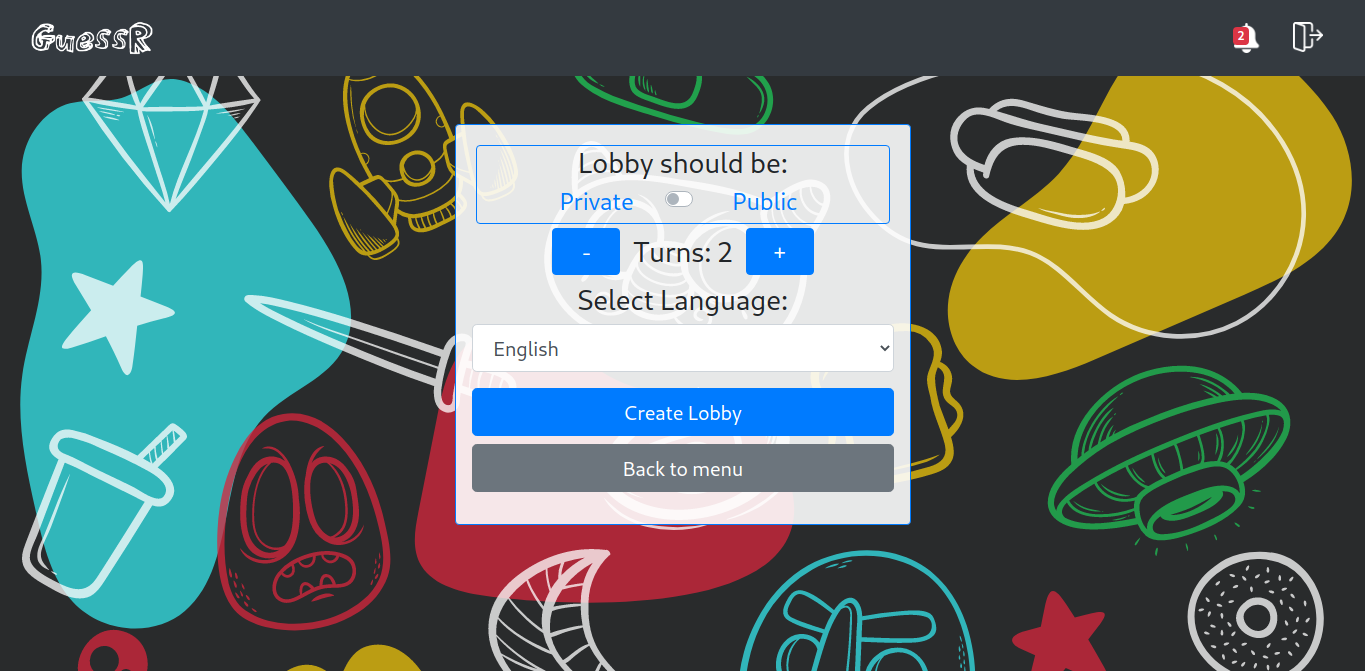
\includegraphics[width=1\linewidth]{img/screen/LobbyCreation.png}
    \caption{Schermata per la creazione di una nuova lobby} 
\end{figure}

Nella schermata per creare una nuova lobby, un utente dovrà specificare la visibilità della lobby (se pubblica e quindi accessibile solo specificando una lingua o privata, quindi accessibile solo se a conoscenza del codice univoco). Successivamente l'utente selezionerà la lingua con cui i partecipanti vorranno comunicare ed il numero di turni di gioco. Una volta creata la lobby, l'utente che ha affrontato il processo di creazione sarà admin della lobby appena creata.

\begin{figure}[H]
  \centering
  \begin{minipage}[b]{0.75\textwidth}
    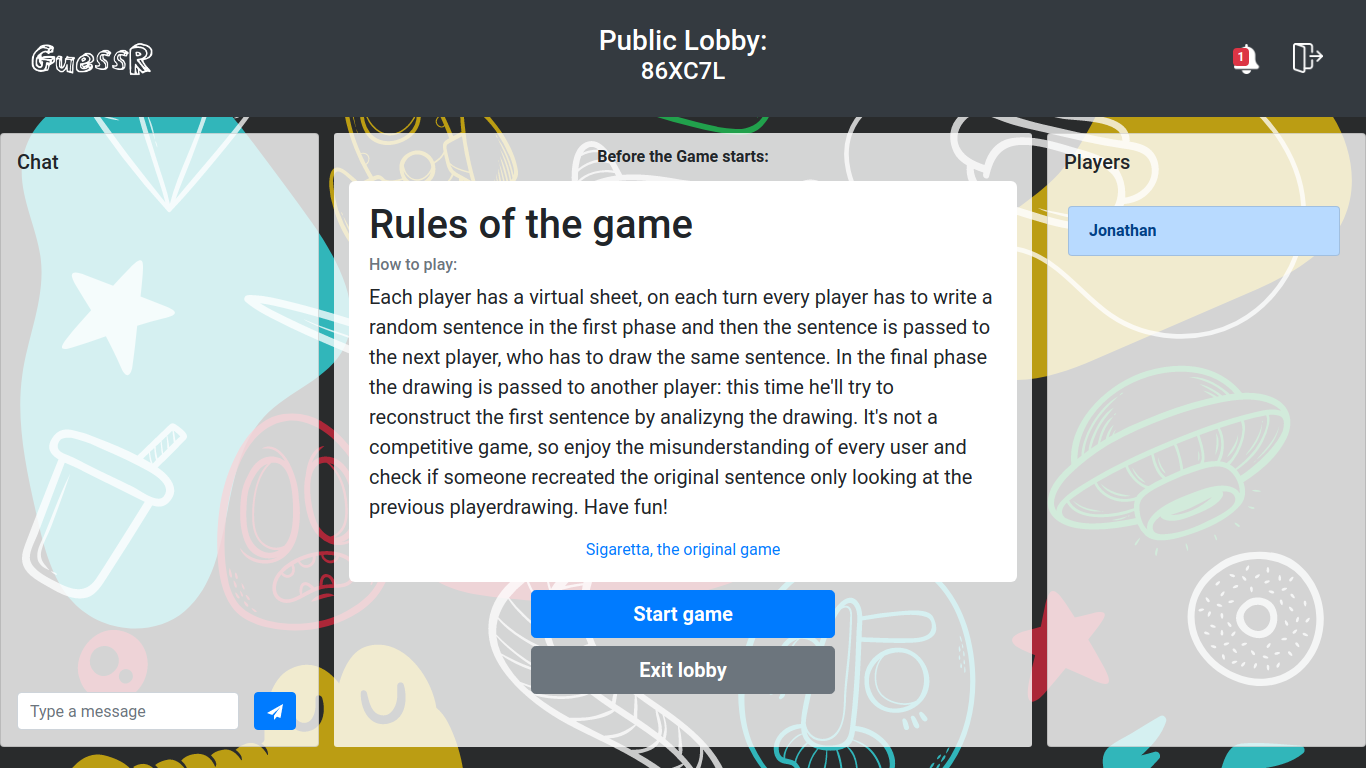
\includegraphics[width=\textwidth]{img/screen/inlobby.png}
  \end{minipage}
  \hfill
  \begin{minipage}[b]{0.2\textwidth}
    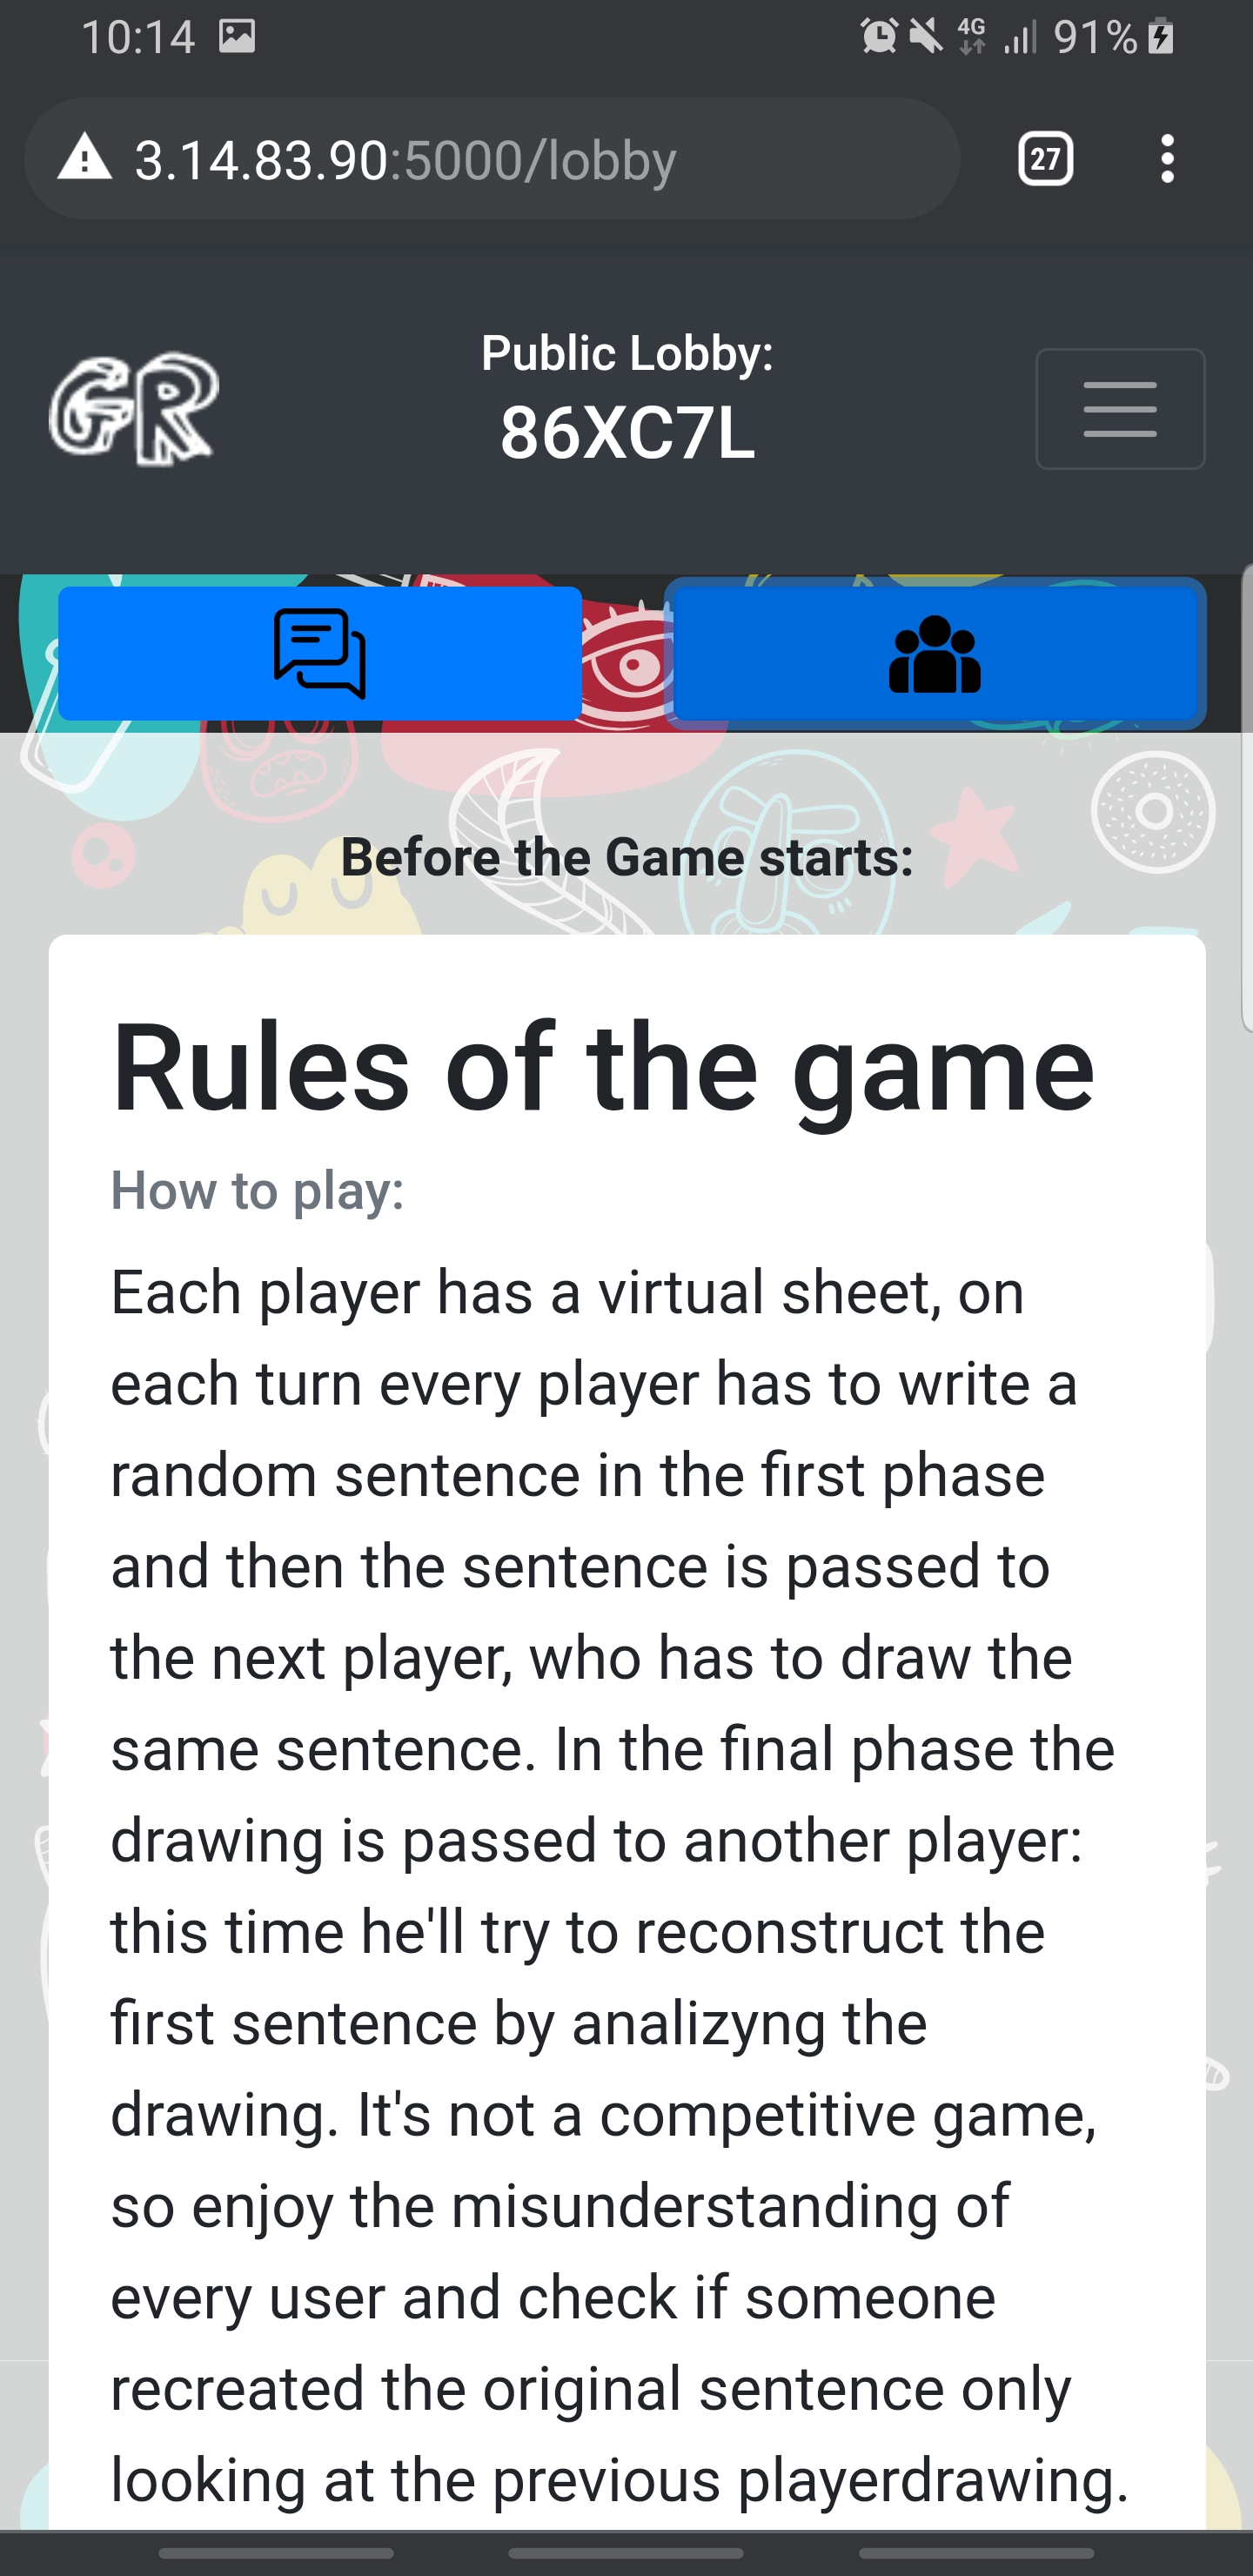
\includegraphics[width=\textwidth]{img/screen/M insideLobby.jpg}
  \end{minipage}
    \caption{Schermate della Lobby (Desktop e Mobile)}
\end{figure}

\noindent La schermata che si visualizza una volta creata una lobby è denominata "insideLobby" e mostra agli utenti una chat, le regole del gioco ed il link alla pagina wikipedia del gioco da cui è tratto GuessR (sigaretta), l'elenco dei membri della lobby ed un pulsante per uscire dalla lobby. Solo l'utente che ha creato la lobby e che quindi ne è amministratore avrà un pulsante per dare il via al vero e proprio gioco. 

 \begin{figure}[H]
  \centering
  \begin{minipage}[b]{0.2\textwidth}
    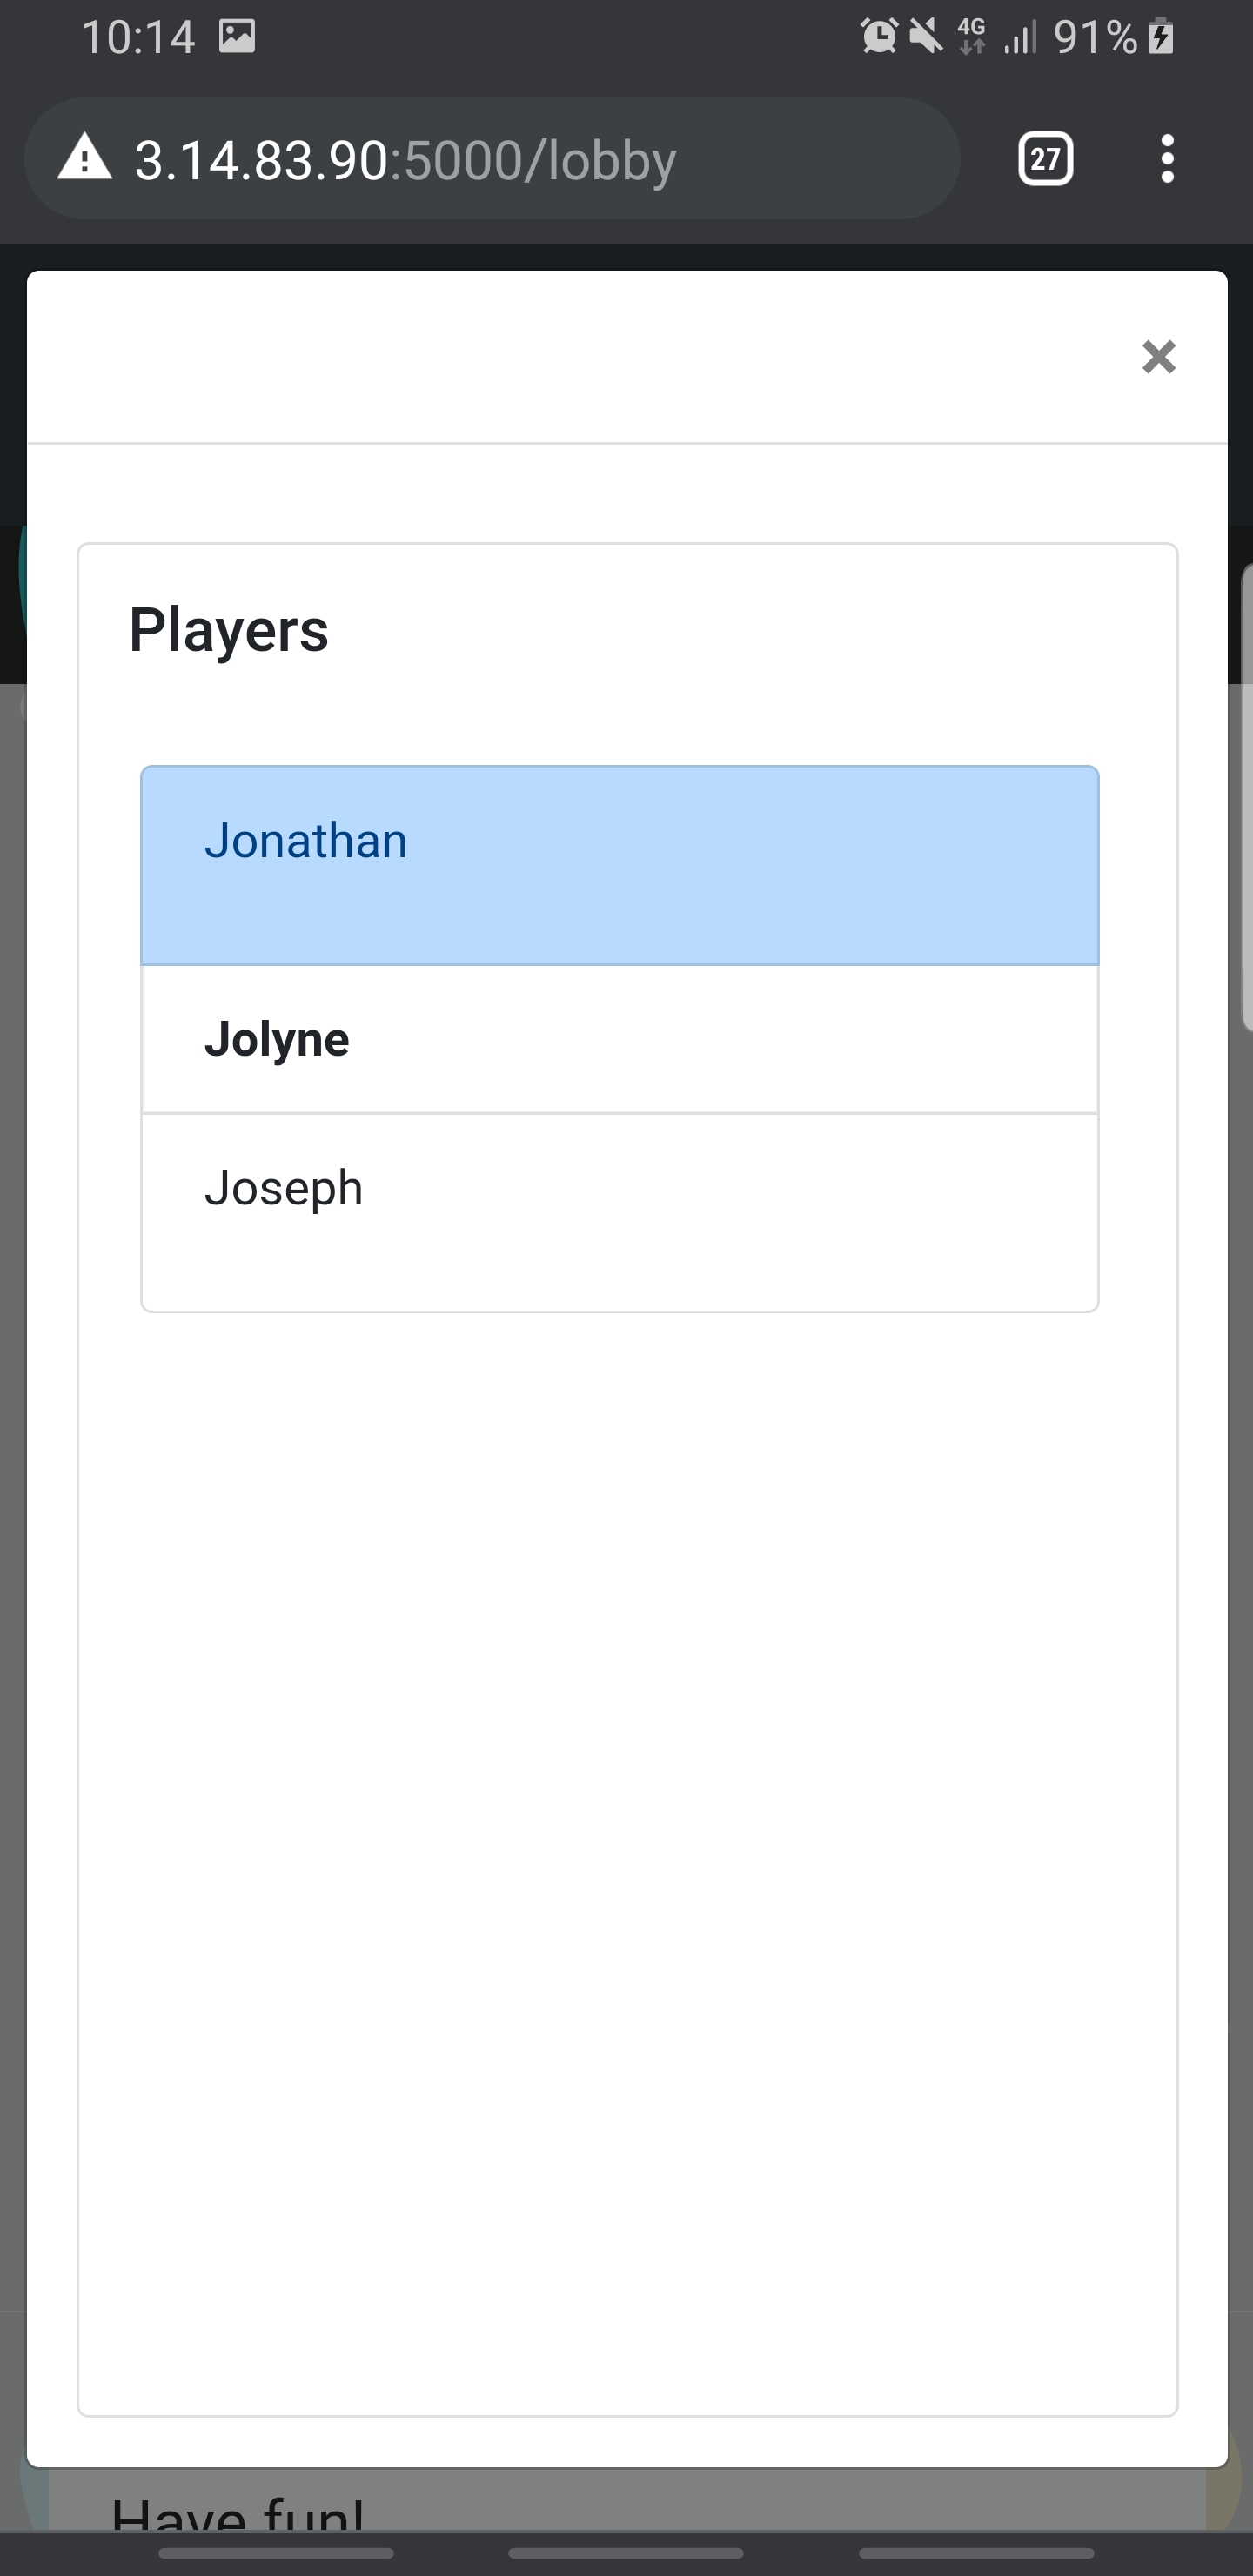
\includegraphics[width=\textwidth]{img/screen/M players.jpg}
  \end{minipage}
  \hspace{1cm}
  \begin{minipage}[b]{0.2\textwidth}
    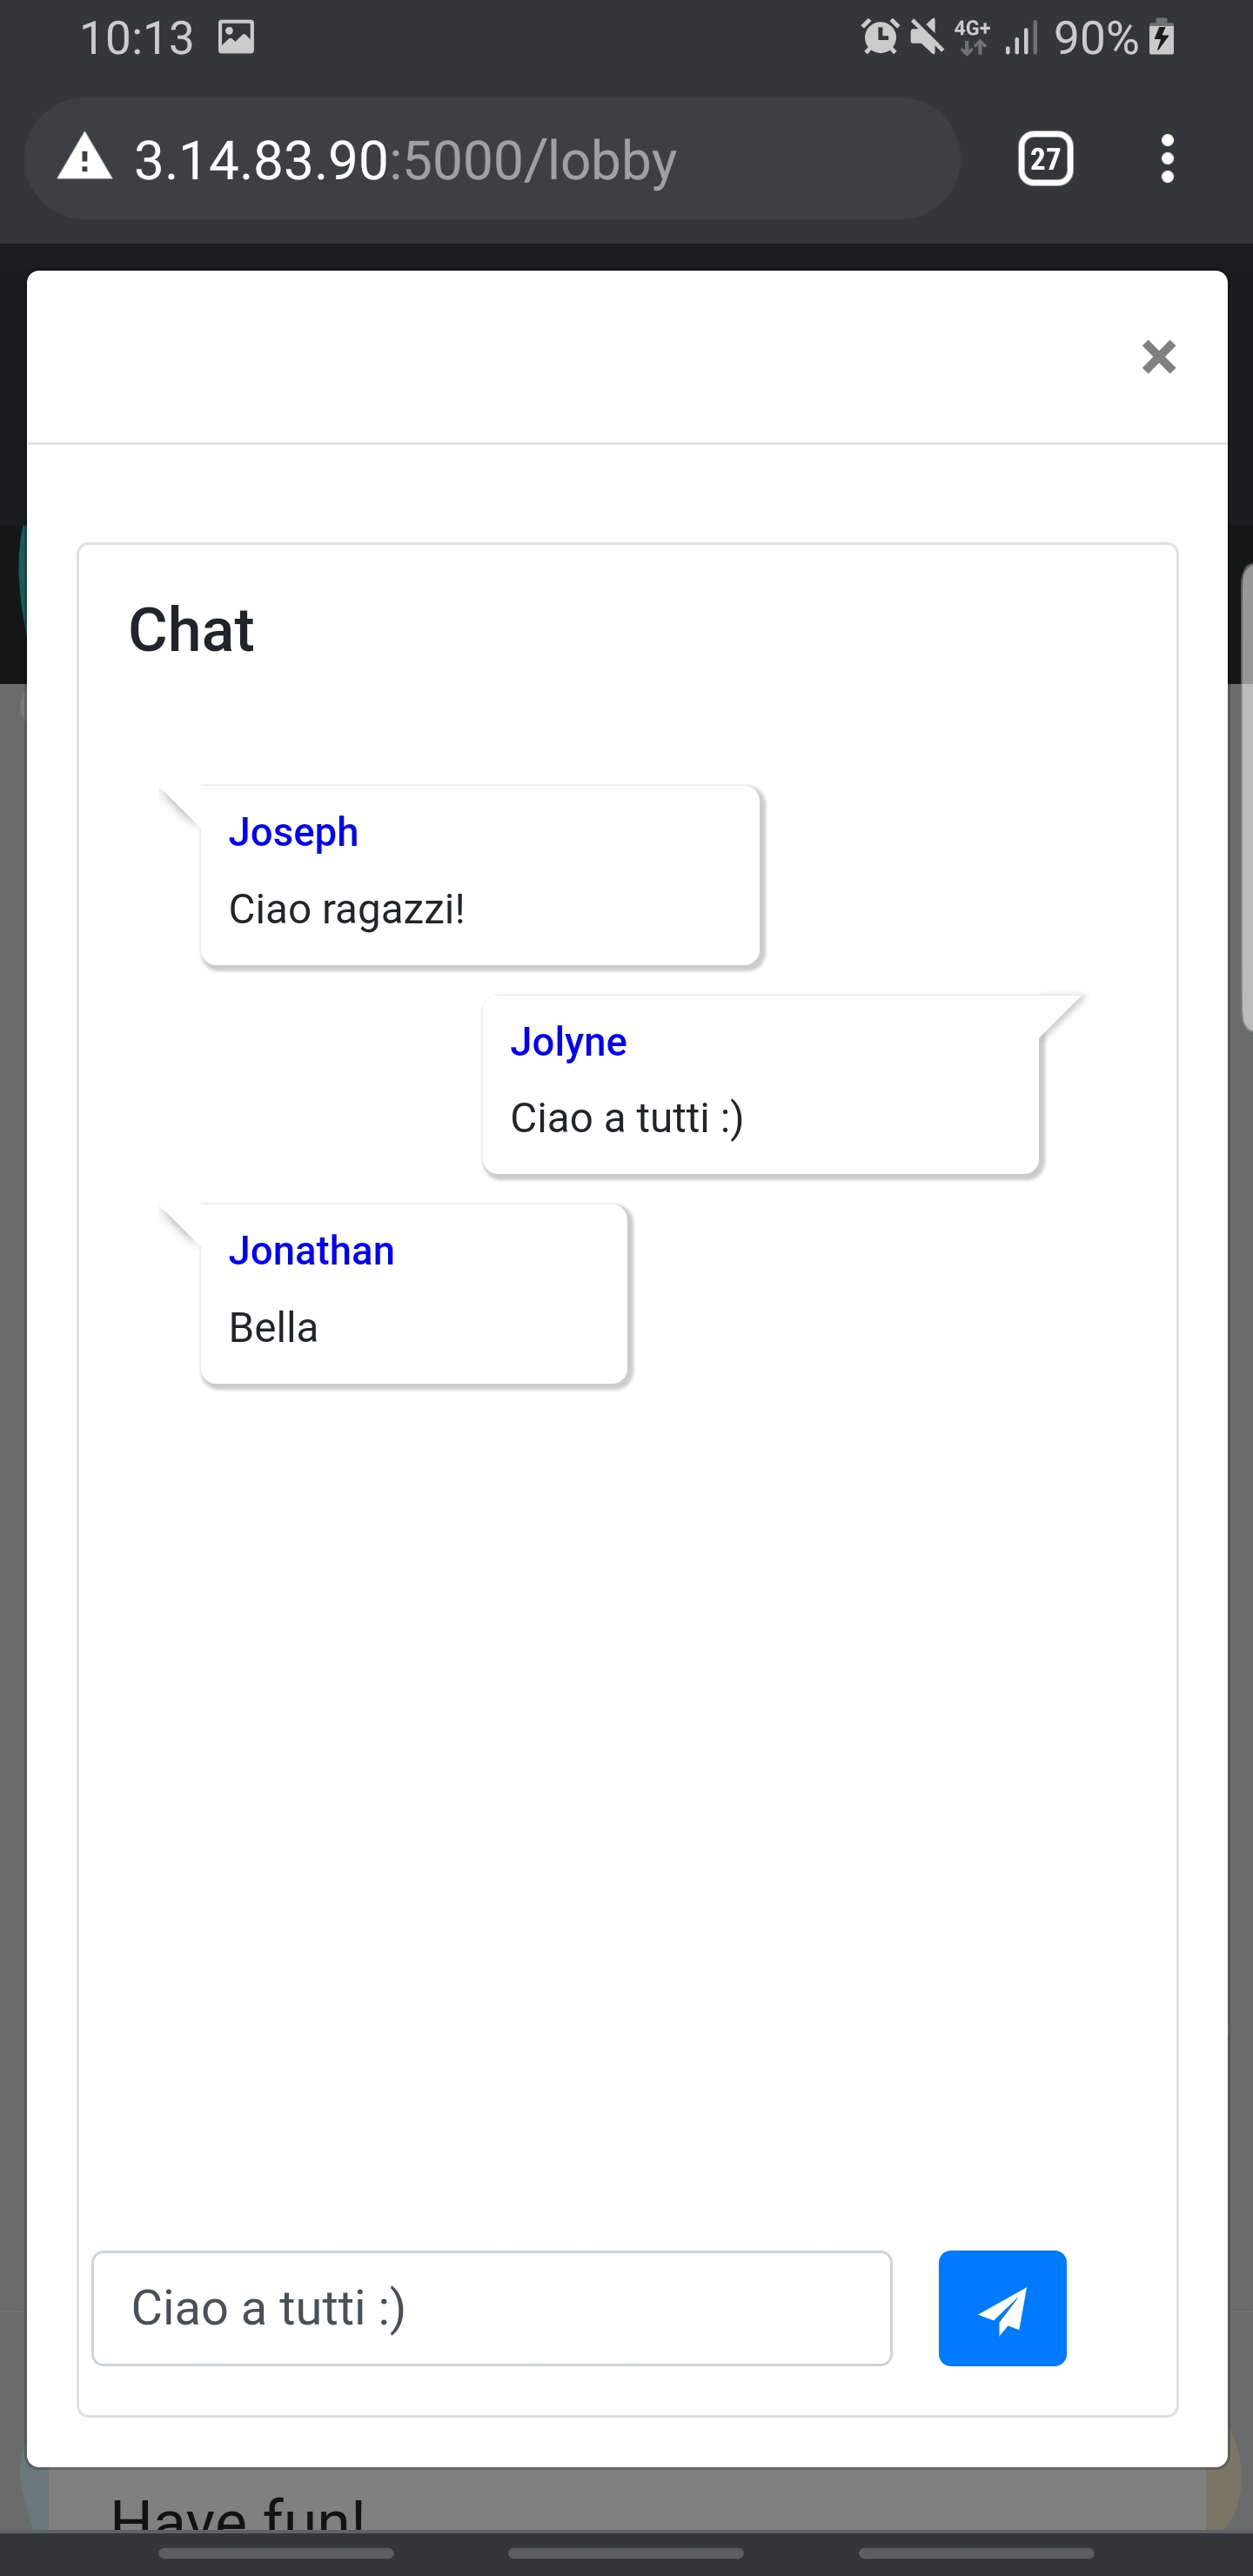
\includegraphics[width=\textwidth]{img/screen/M chat.jpg}
  \end{minipage}
    \caption{Schermate Mobile di Chat e Giocatori}
\end{figure}

\noindent Nella visualizzazione mobile i pannelli relativi alla chat ed ai giocatori sono collassati in due pulsanti presenti sotto da navbar, nella parte superiore dello schermo.


\begin{figure}[H]
    \centering
    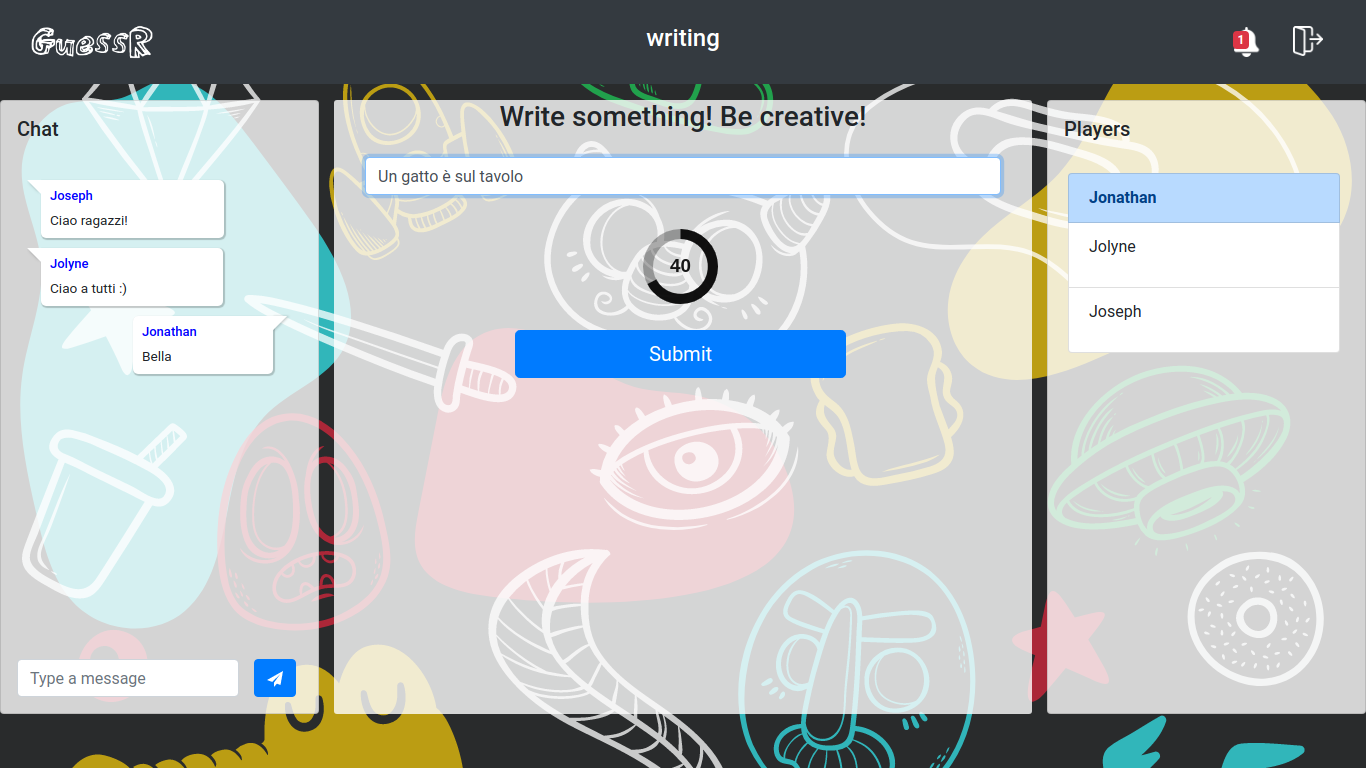
\includegraphics[width=0.8\linewidth]{img/screen/sentence (1).png}
    \caption{Schermata di sentence} 
\end{figure}

\noindent Una volta avviato il gioco la prima fase in cui ogni giocatore si trova è quella di "sentence", che vede l'inserimento di una frase scelta dal giocatore. Ogni giocatore sia nella fase di sentence che in quella di draw avrà un timer sincronizzato ad indicargli di quanto tempo dispone prima che ciò che ha scritto/disegnato venga sottoposto automaticamente.

 \begin{figure}[H]
  \centering
  \begin{minipage}[b]{0.75\textwidth}
    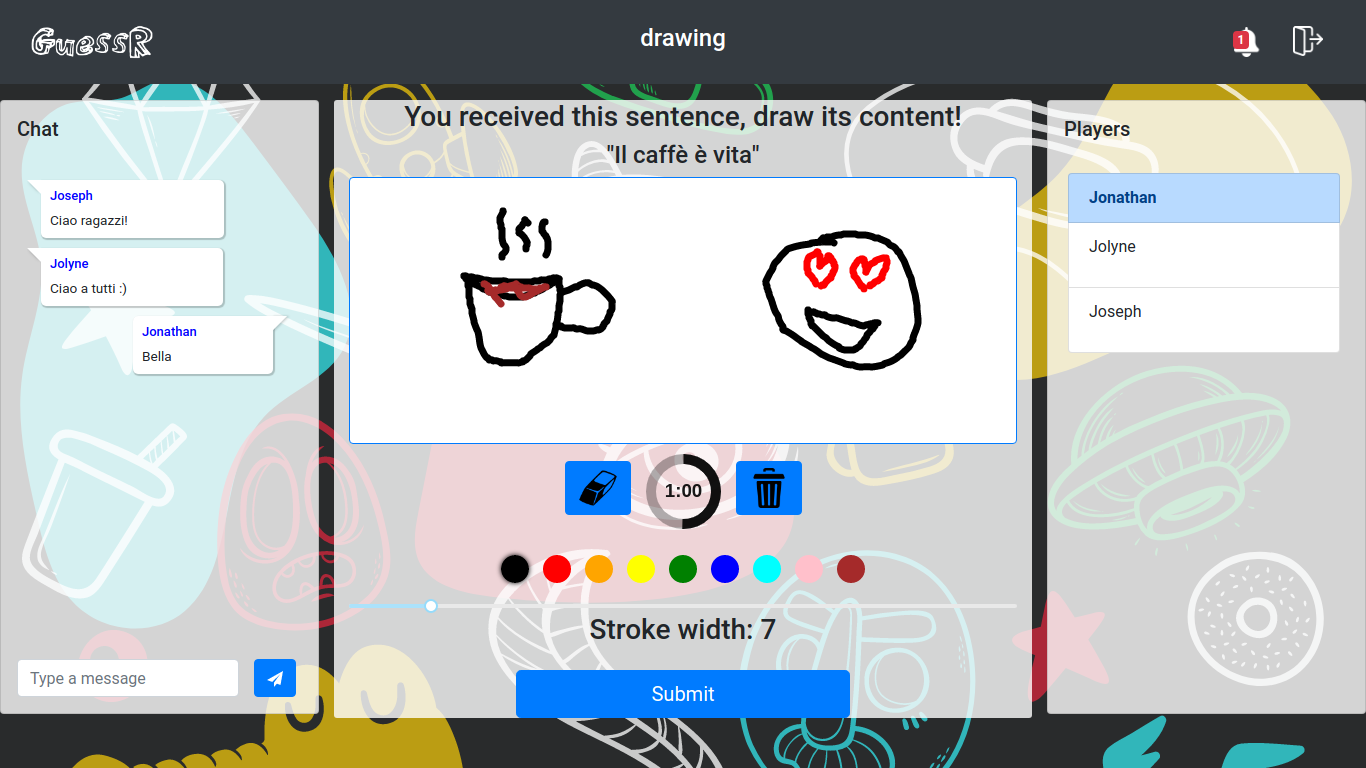
\includegraphics[width=\textwidth]{img/screen/draw_1.png}
  \end{minipage}
  \hfill
  \begin{minipage}[b]{0.2\textwidth}
    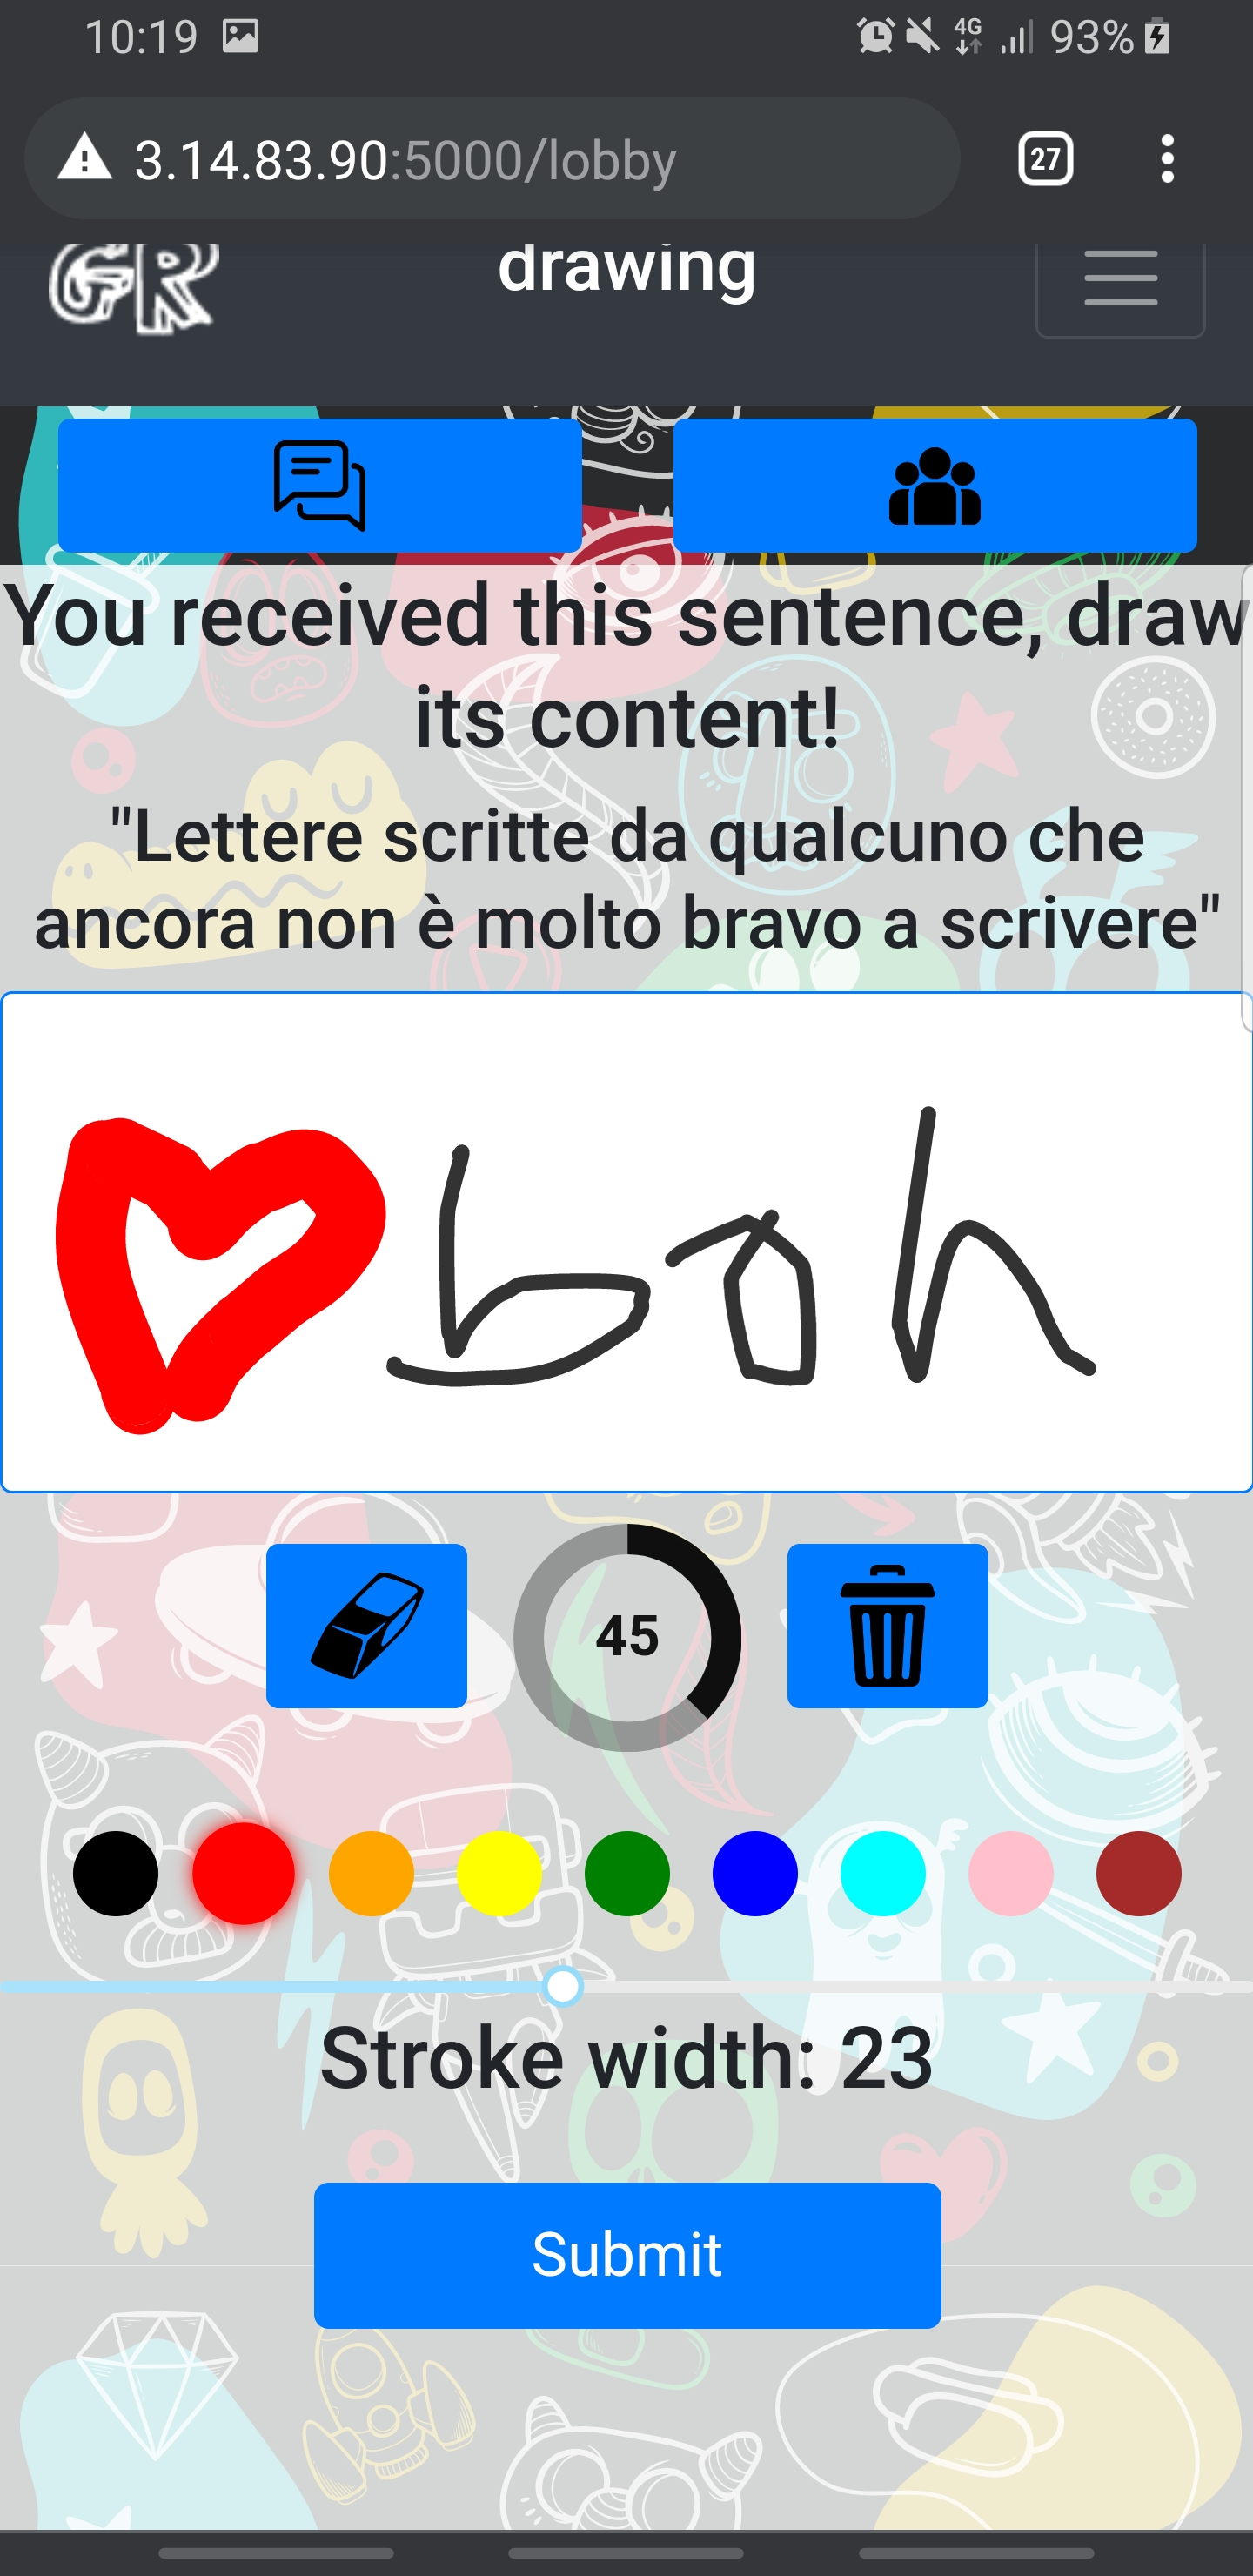
\includegraphics[width=\textwidth]{img/screen/M draw.jpg}
  \end{minipage}
    \caption{Schermate di Disegno (Desktop e Mobile)}
\end{figure}

\noindent Nella fase di "draw", a gli utenti viene predisposto un canvas centrale su cui possono disegnare la frase che gli spetta, oltre al timer questa volta gli utenti hanno una suite di strumenti da utilizzare per il disegno, come una serie di diversi colori, una gomma ed un pulsante per resettare il canvas e uno slider che gli permette di impostare lo spessore del tratto da utilizzare.



\begin{figure}[H]
    \centering
    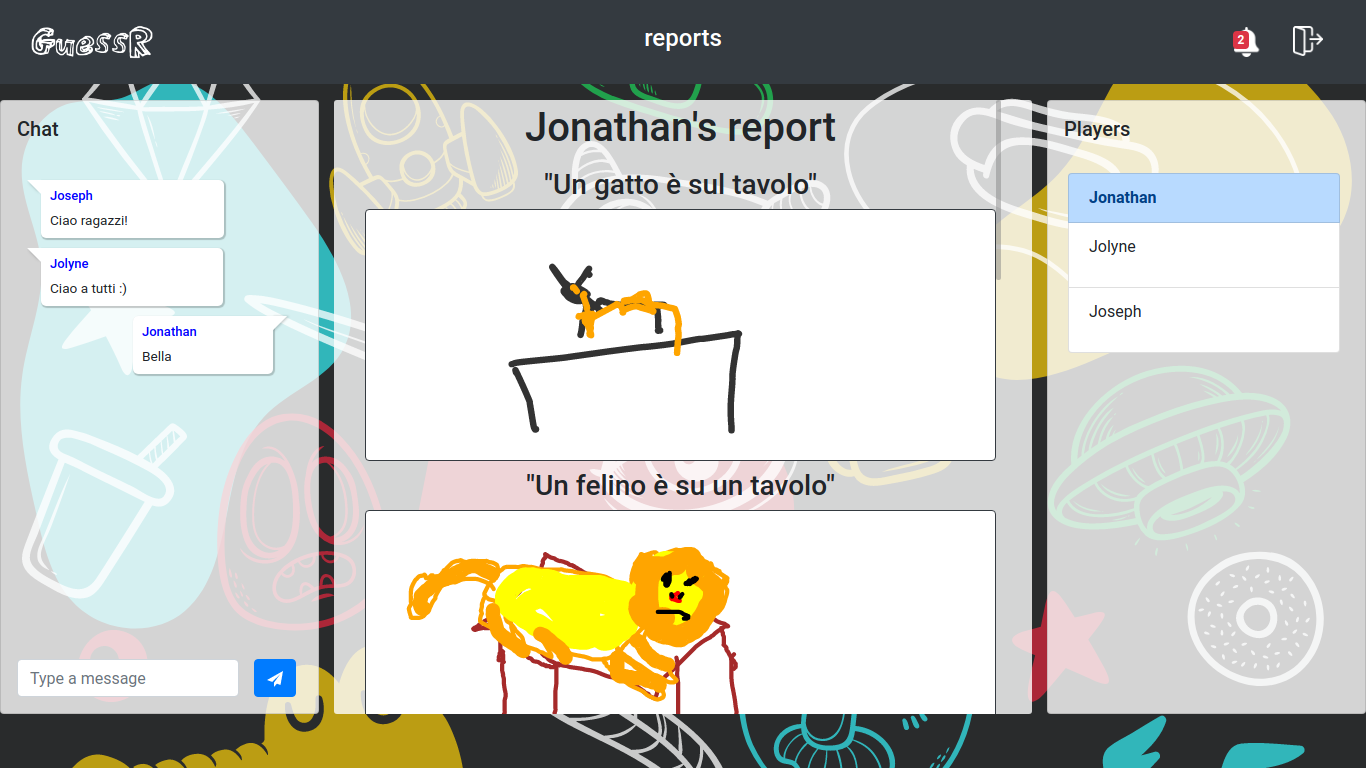
\includegraphics[width=0.8\linewidth]{img/screen/end_report_1.png}
    \caption{Schermata dei Report finale} 
\end{figure}

\noindent Una volta terminato il gioco a seconda dei turni impostati in fase di creazione della lobby, i giocatori si ritrovano nella schermata di "show reports" in cui trovano un resoconto della partita appena svolta e l'evoluzione di ogni frase e disegno. Questa è la fase in cui i giocatori si confrontano, o in chat vocale separata o utilizzando la chat predisposta da GuessR per commentare la partita appena terminata.

 \begin{figure}[H]
  \centering
  \begin{minipage}[b]{0.73\textwidth}
    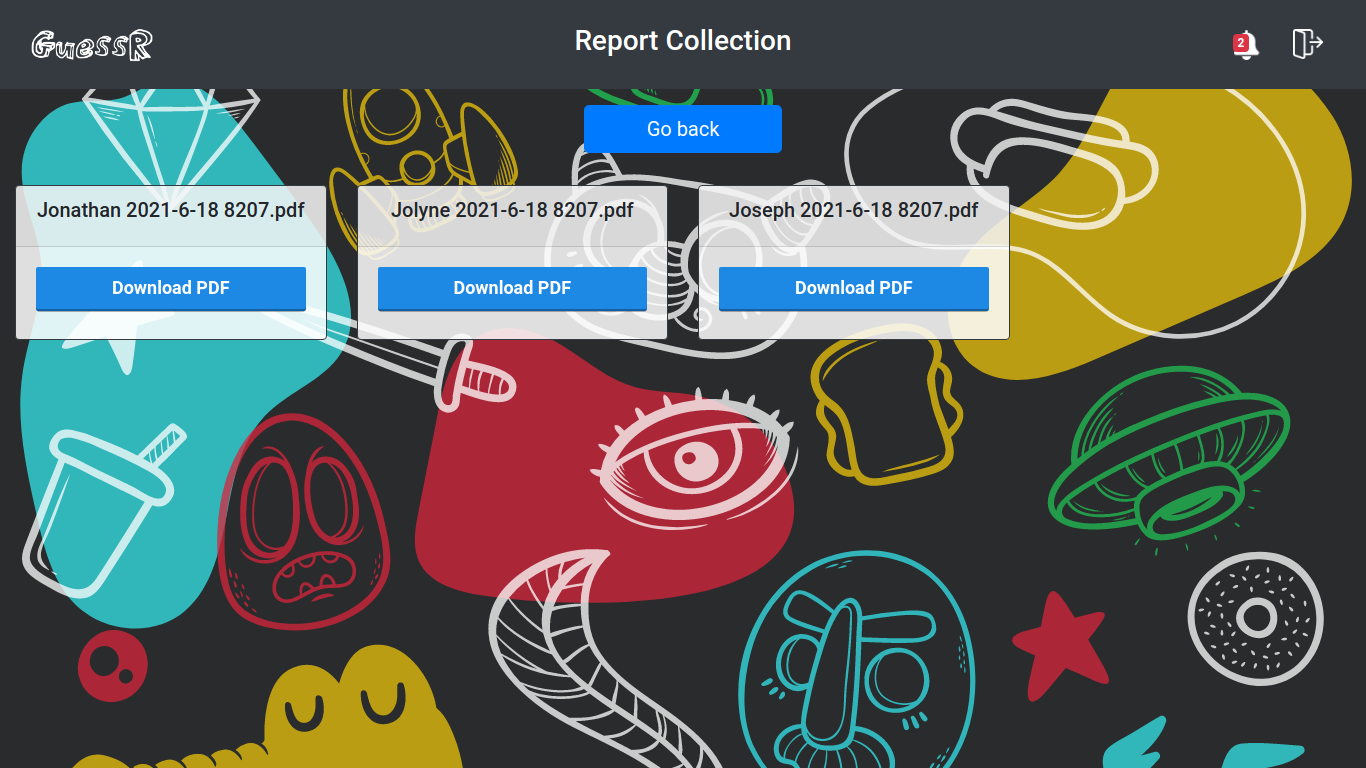
\includegraphics[width=\textwidth]{img/screen/previous_reports.png}
  \end{minipage}
  \hspace{1cm}
  \begin{minipage}[b]{0.19\textwidth}
    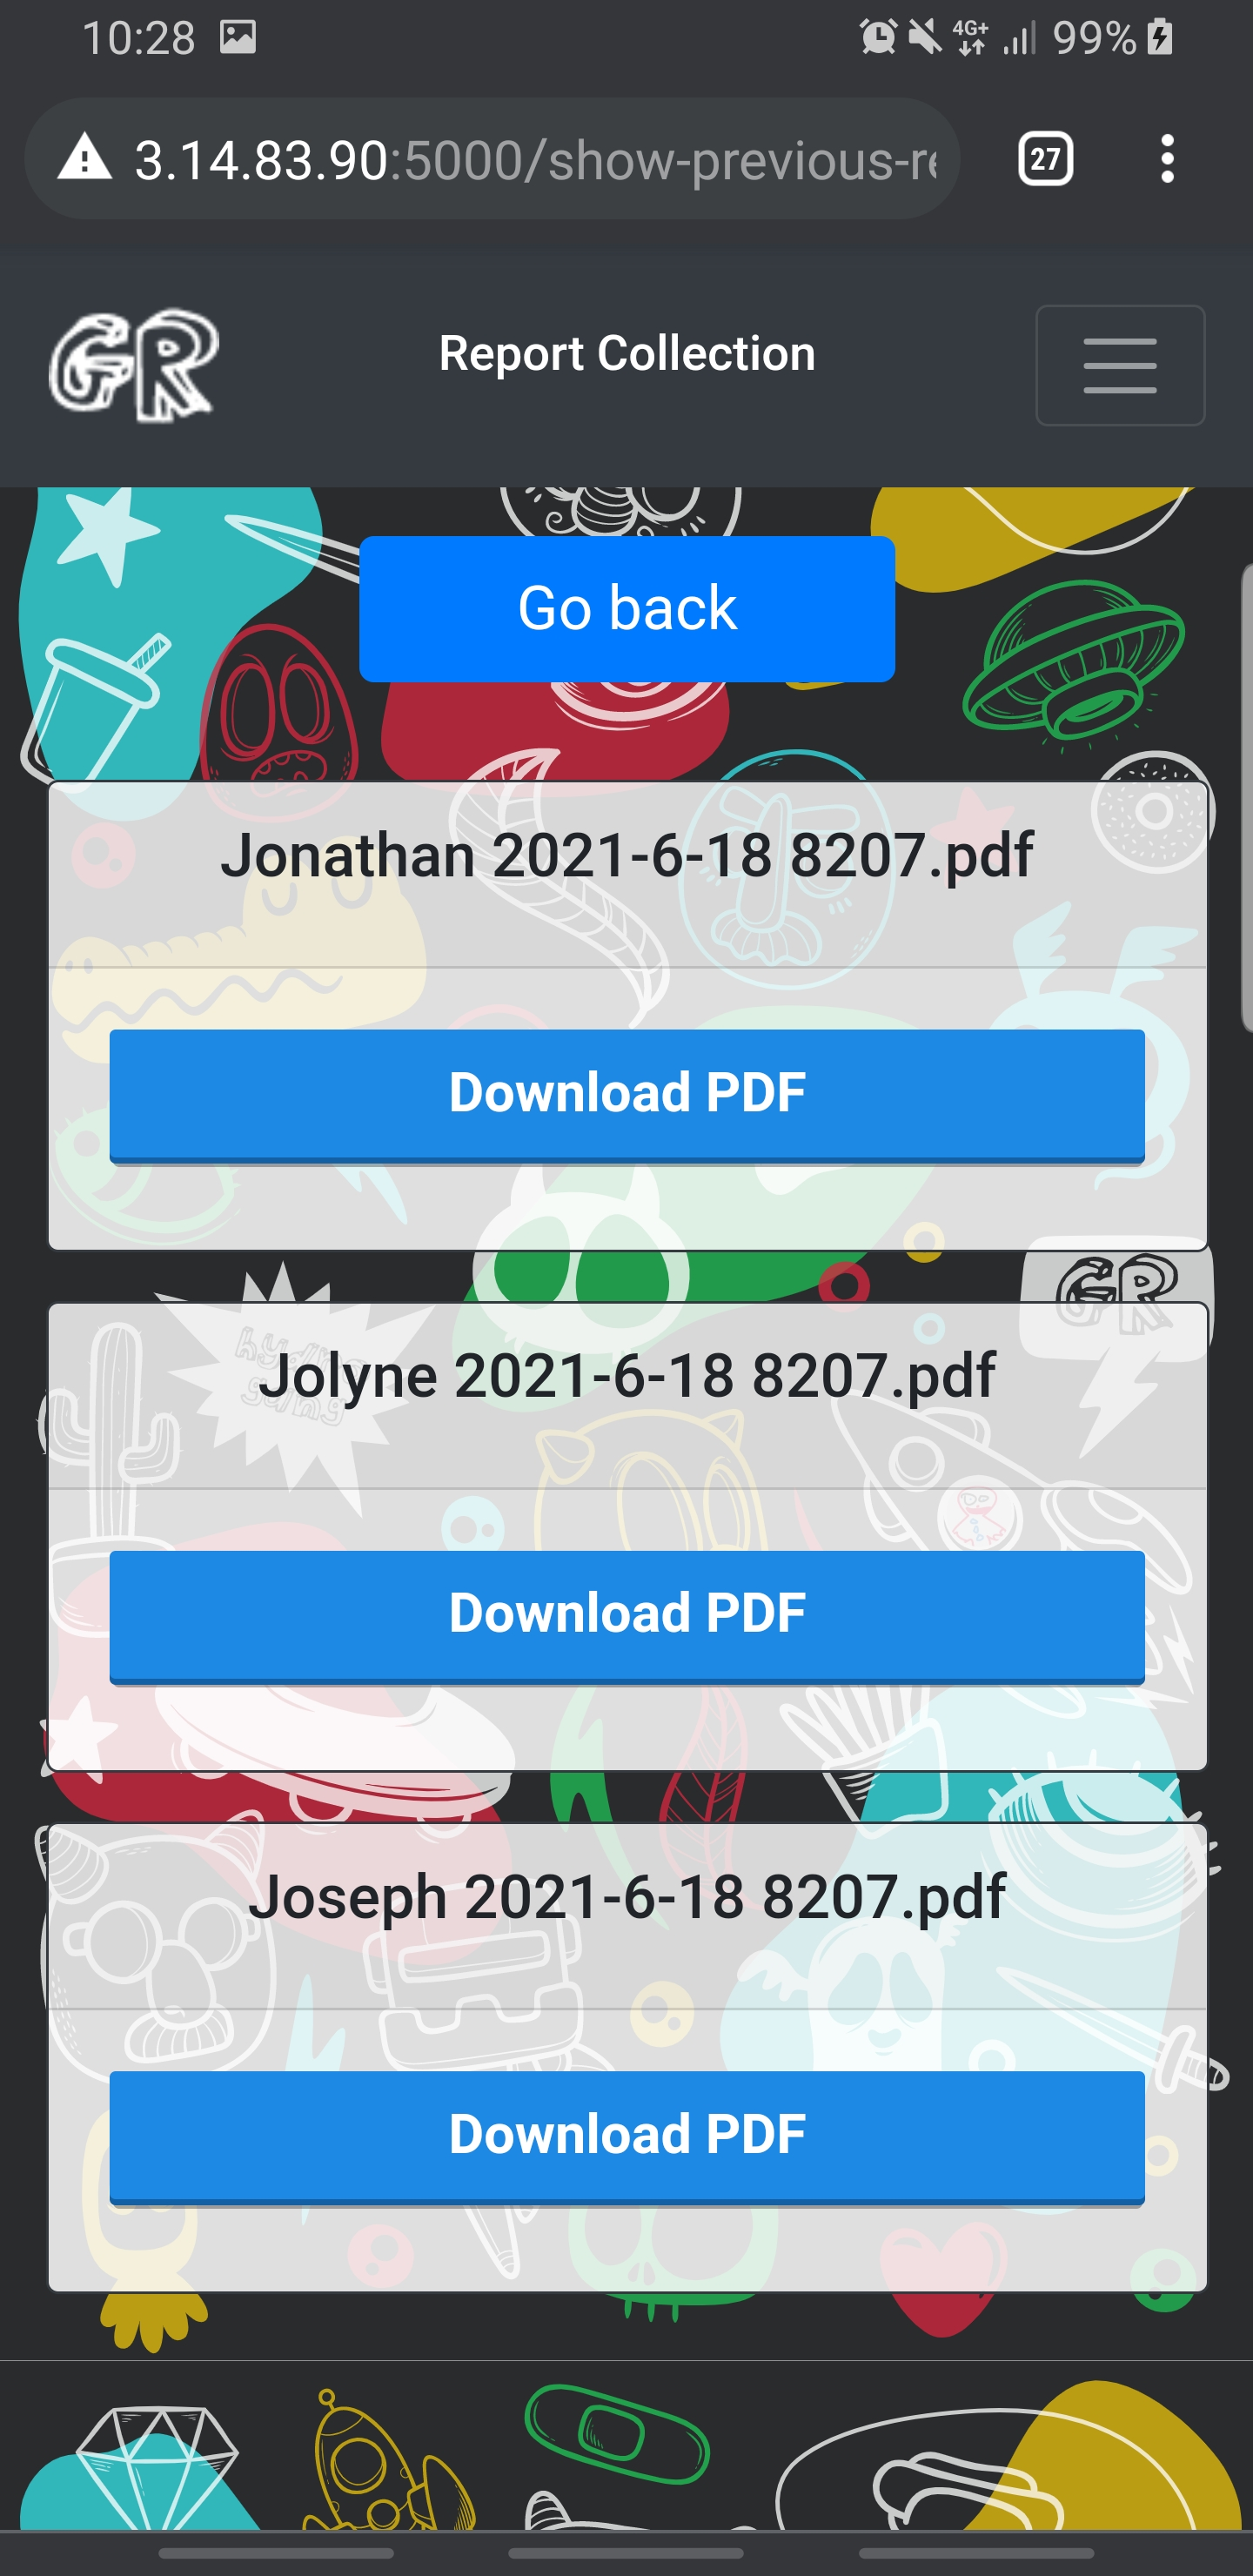
\includegraphics[width=\textwidth]{img/screen/M reports.jpg}
  \end{minipage}
    \caption{Schermata dei report precedenti (Desktop e Mobile)}
\end{figure}

Gli utenti che hanno svolto delle partite possono accedere in ogni momento ad una interfaccia apposita predisposta per consultare e scaricare i report di partite precedenti, identici a quelli visualizzati al termine della partita.

 \begin{figure}[H]
  \centering
  \begin{minipage}[b]{0.73\textwidth}
    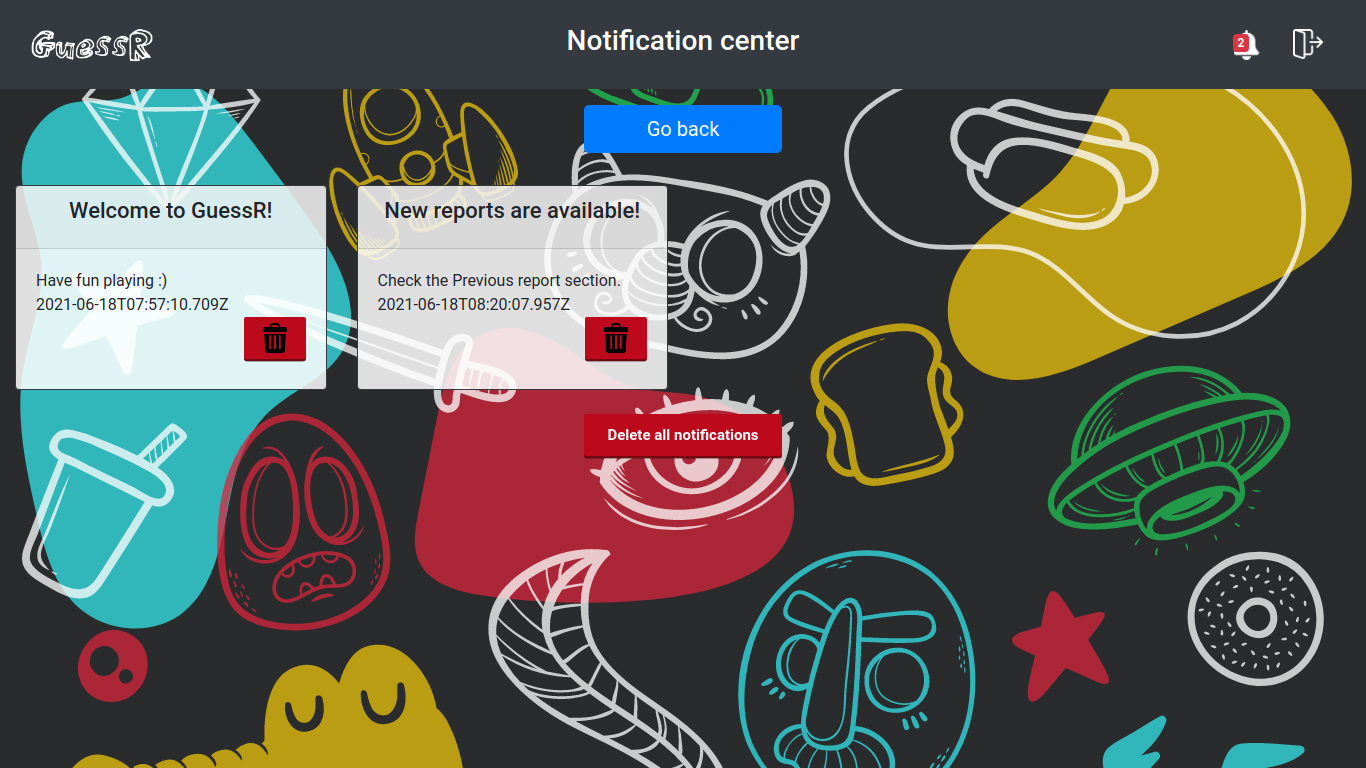
\includegraphics[width=\textwidth]{img/screen/notifications.png}
  \end{minipage}
  \hspace{1cm}
  \begin{minipage}[b]{0.19\textwidth}
    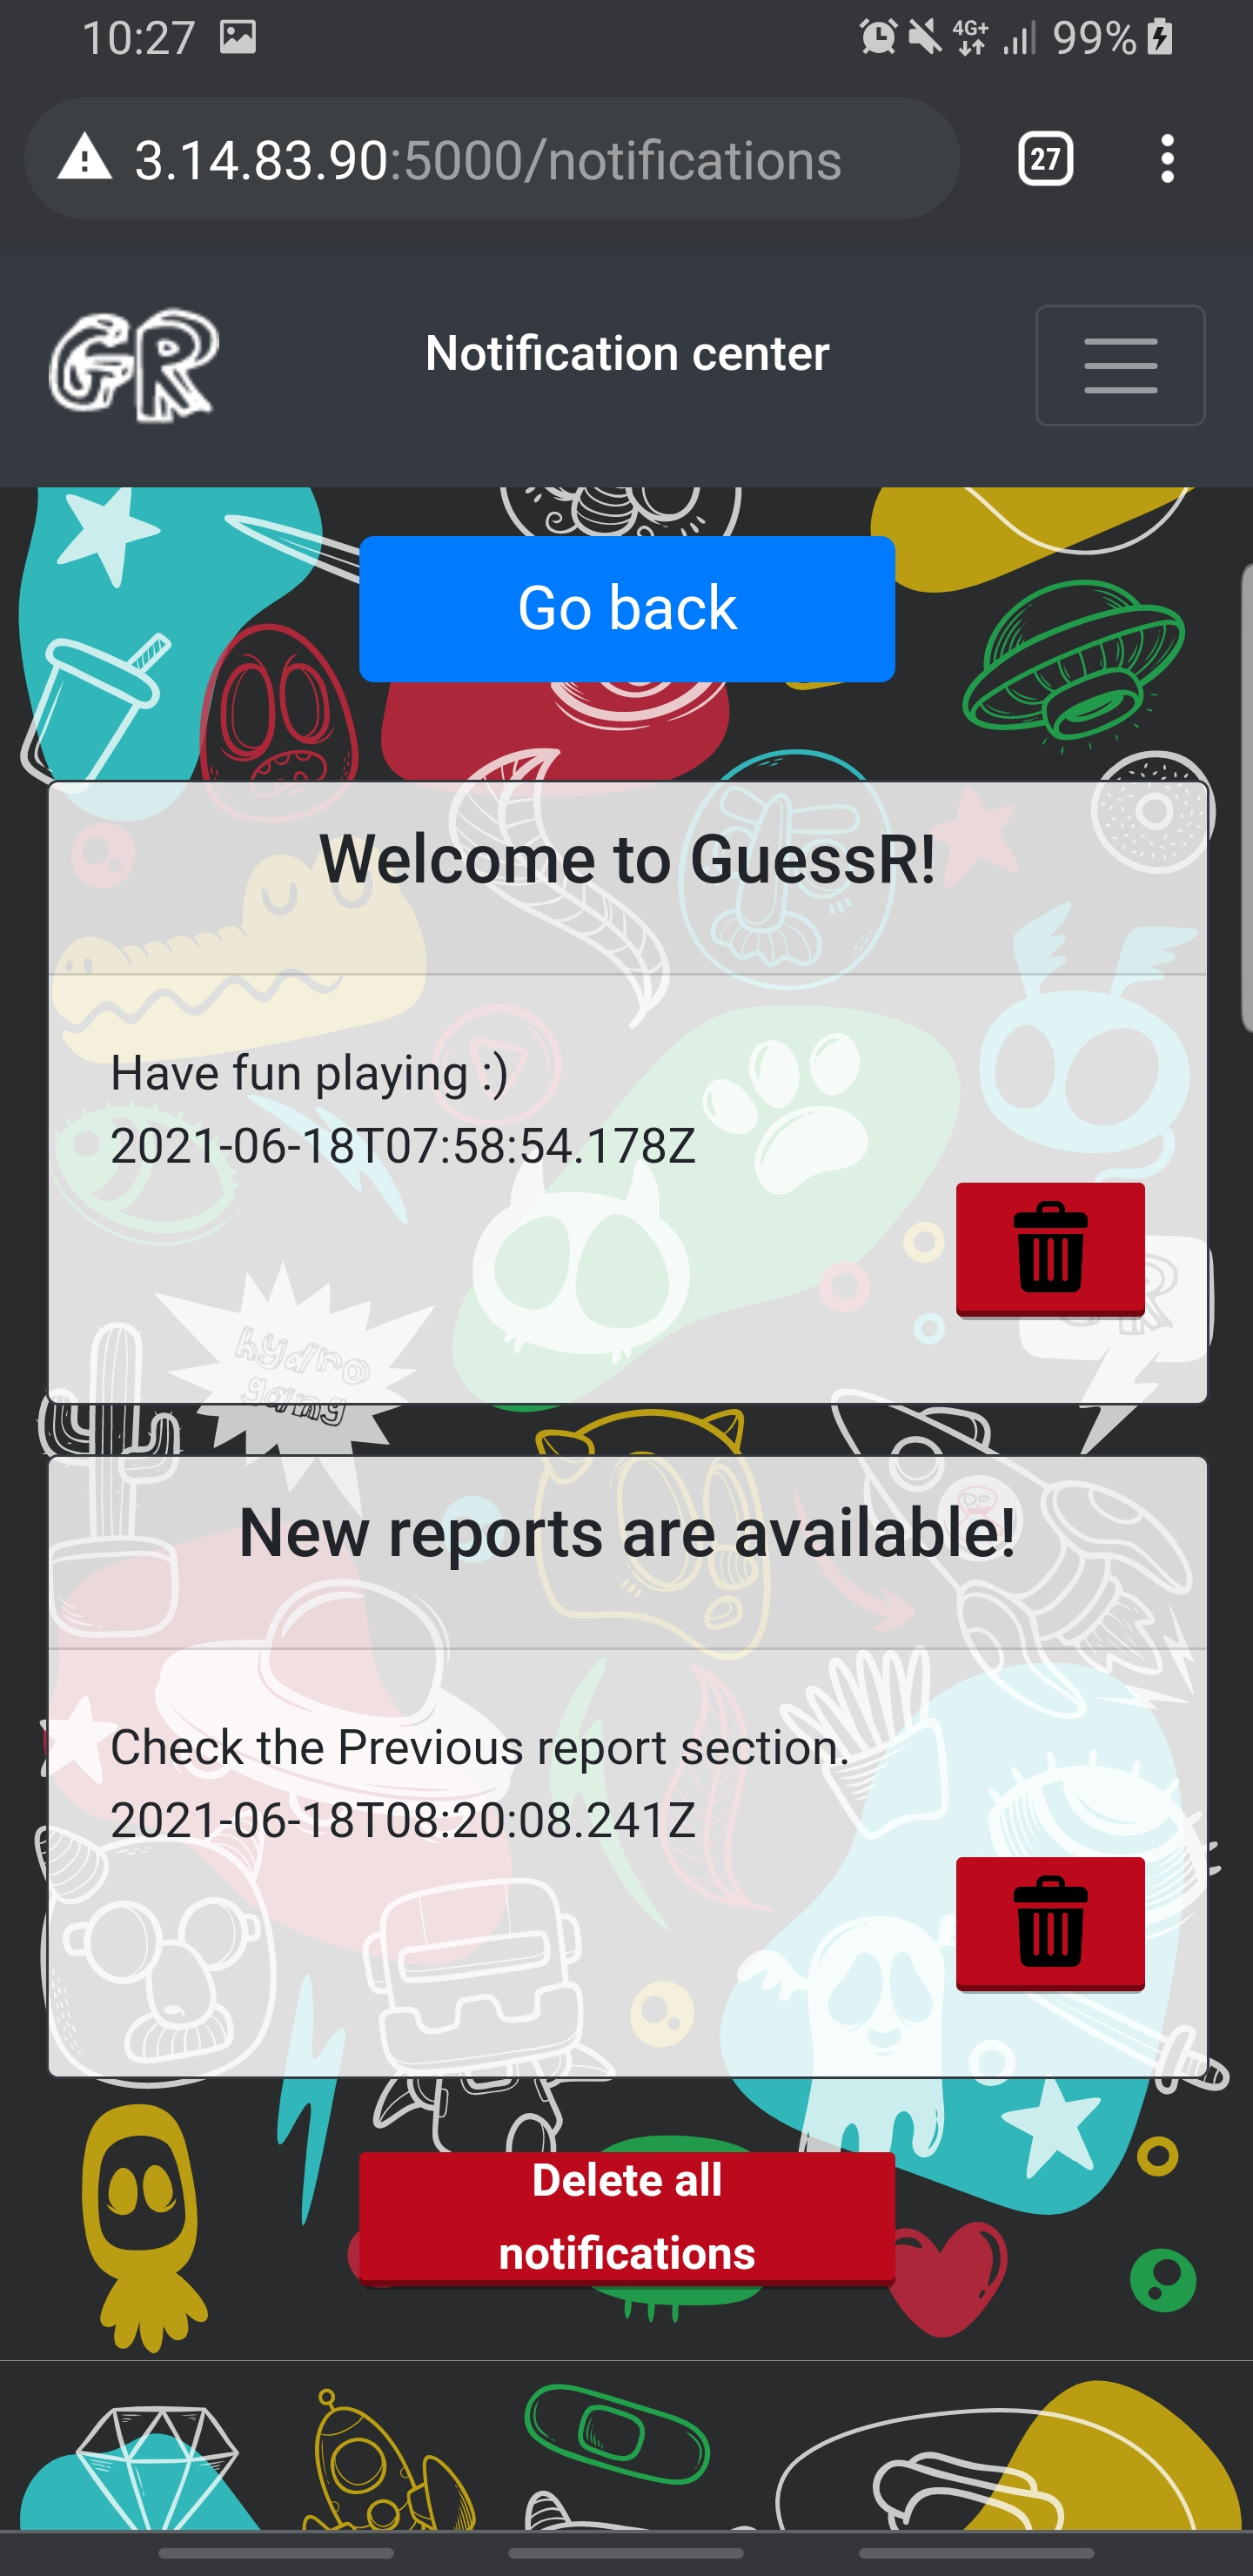
\includegraphics[width=\textwidth]{img/screen/M notifications.jpg}
  \end{minipage}
    \caption{Schermate delle notifiche (Desktop e Mobile)}
\end{figure}

Gli utenti possono in ogni momento consultare la pagina relative alle notifiche, che se presenti si mostrano con un badge rosso contenente il numero di notifiche ricevute, nell'apposita icona presente sulla navbar. 

\begin{figure}[H]
    \centering
    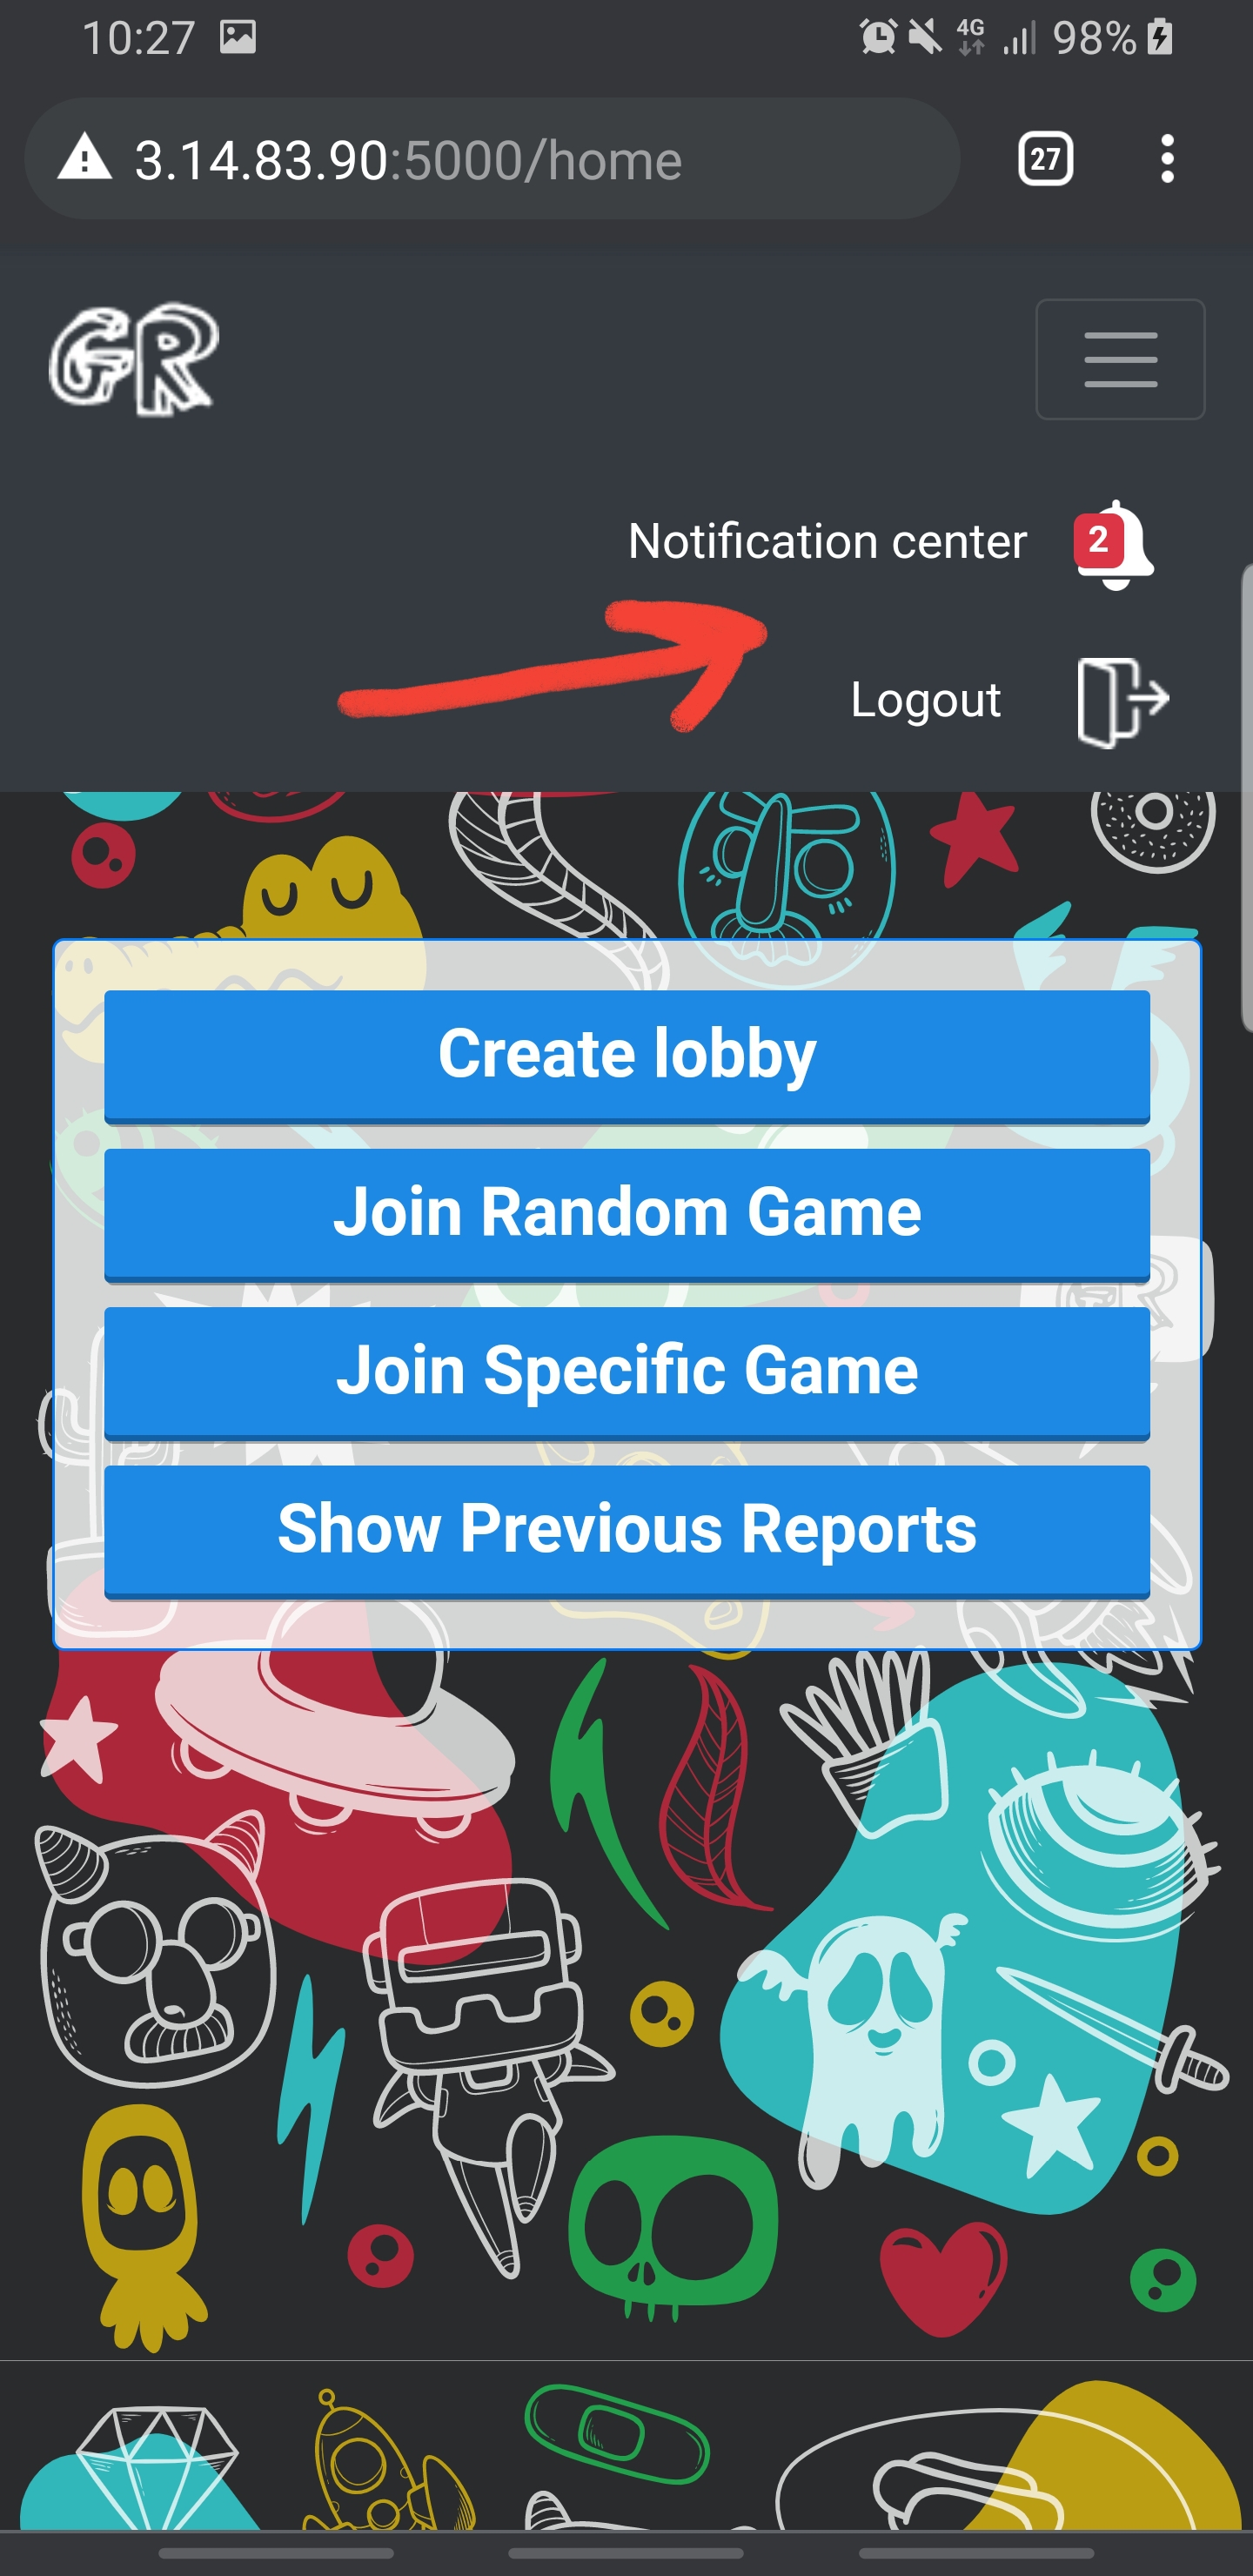
\includegraphics[width=0.3\linewidth]{img/screen/M notification Pointer.jpg}
    \caption{Schermata mobile contenente la navbar ed il menù a dropdown} 
\end{figure}

Nella versione mobile l'icona di notifiche e di logout sono collassate in un menù a dropdown per favorire la responsiveness del sito e conferire una miglior UX.


\subsection{Scelte estetiche e UI}

\begin{figure}[H]
    \centering
    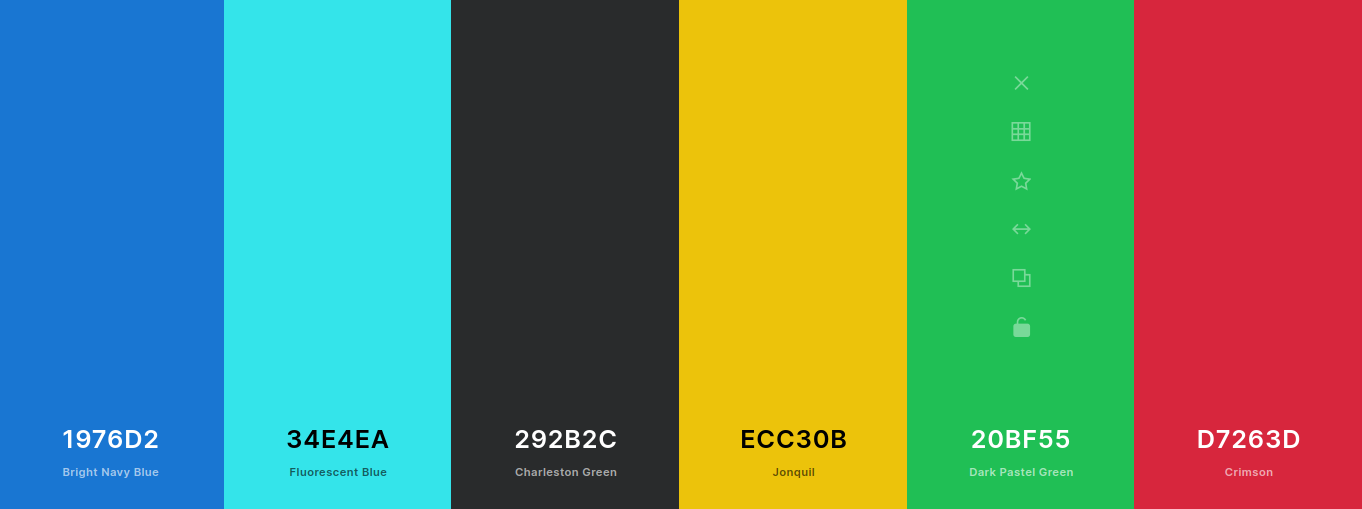
\includegraphics[width=0.9\linewidth]{img/screen/Palette.png}
    \caption{Palette di colori utilizzata per i componenti del sito, il logo e lo sfondo} 
\end{figure}

\noindent Lo sfondo, i colori e le trasparenze sono stati scelti in modo da rendere il sito quanto più gradevole alla vista ma mantenendo sempre come primo obiettivo la leggibilità, l'accessibilità e la scalabilità del sito. Ogni schermata è stata validata da appositi strumenti allo scopo di verificare che i colori adottati dalla palette e presenti nel sito non ostacolino in alcun modo la leggibilità, nemmeno nel caso di persone ipovedenti. Lo sfondo svolge un duplice ruolo, contenendo numerosi disegni e forme funge anche da fonte di ispirazione per utenti che si ritrovano a dover disegnare qualcosa, alcuni dei disegni presenti sullo sfondo sono stati effettuati in fase di testing del gioco con veri utenti.

\begin{figure}[H]
    \centering
    
\includegraphics[width=0.4\linewidth]{img/screen/logoHover.png}
    \caption{Logo di GuessR} 
\end{figure}

\noindent Il logo nella sua versione estesa riporta il nome del gioco "GuessR" in un font che ricorda un disegno effettuato a mano libera e varia nel formato desktop quando viene effettuato un hover. Nella versione mobile riporta le lettere "GR".